% =============================================================================
% CAPÍTULO 2: INTELIGÊNCIA ARTIFICIAL E ARQUITETURA DE AGENTES COGNITIVOS
% Níveis: 0 (zero) ao PhD
% Autor: Marcelo Claro Laranjeira
% =============================================================================
\chapter{Inteligência Artificial e Arquitetura de Agentes Cognitivos}
\label{cap:inteligencia-artificial-agentes}

\paragraph{O cérebro do ecossistema.} Se o Capítulo~1 forneceu a matemática
--- a ``linguagem'' com a qual descrevemos e analisamos sistemas ---, este
capítulo apresenta o ``cérebro'': a inteligência artificial e as arquiteturas
de agentes que dão vida ao \opencodeeco{}. Aqui exploraremos como máquinas
podem aprender, raciocinar e agir de forma autônoma.

A inteligência artificial (IA) deixou de ser uma promessa futurista para se
tornar o motor central da transformação digital contemporânea. Dos assistentes
virtuais aos sistemas de recomendação, dos carros autônomos aos agentes de
código que escrevem software, a IA permeia todas as camadas da tecnologia
moderna \cite{russell2020inteligencia, lecun2015deep}.
Este capítulo apresenta os fundamentos da inteligência artificial com ênfase
em arquiteturas de agentes cognitivos --- o alicerce sobre o qual o
\opencodeeco{} foi construído. Percorreremos uma jornada que se inicia nos
primórdios da IA, atravessa o aprendizado de máquina e as redes neurais
profundas, e culmina nos sistemas multiagentes e motores de raciocínio formal
que equipam o ecossistema com 128 agentes, 227 skills e 46 MCPs.
A Tabela~\ref{tab:conteudo-capitulo2} apresenta a estrutura do capítulo com
os níveis de dificuldade e carga horária estimada.
\begin{table}[htb]
\centering
    \small
\caption{Conteúdo do Capítulo 2}
\label{tab:conteudo-capitulo2}
    \resizebox{\textwidth}{!}{
\begin{tabular}{clcc}
\toprule
\textbf{Seção} & \textbf{Tópico} & \textbf{Nível} & \textbf{Estudo} \\
\midrule
2.1 & Fundamentos de IA & \nivelzero & 8h \\
2.2 & Aprendizado de Máquina & \nivelbasico & 10h \\
2.3 & Redes Neurais e Deep Learning & \nivelintermediario & 12h \\
2.4 & Transformers e LLMs & \nivelavancado & 12h \\
2.5 & Engenharia de Prompts e Raciocínio & \nivelavancado & 8h \\
2.6 & Sistemas Multiagentes & \nivelavancado & 10h \\
2.7 & Motores de Raciocínio Formal & \nivelphd & 8h \\
2.8 & Agentes Autônomos e Ciclo Percepção-Ação & \nivelphd & 6h \\
2.9 & Integração Prática no \opencodeeco{} & \text{Todos} & 6h \\
\bottomrule
\end{tabular}
    }
\end{table}
% =============================================================================
% SEÇÃO 2.1: FUNDAMENTOS DE INTELIGÊNCIA ARTIFICIAL
% Nível: 0 (zero) / Básico (~8 laudas)
% =============================================================================
\section{Fundamentos de Inteligência Artificial}
\label{sec:fundamentos-ia}
\nivelzero

\paragraph{Como ensinar máquinas a pensar?} O que significa uma máquina ser
``inteligente''? É executar instruções pré-programadas ou aprender com a
experiência? Esta seção percorre as origens da IA, desde o Teste de Turing
até o debate entre abordagens simbólicas e conexionistas --- duas visões que
o \opencodeeco{} combina em sua arquitetura híbrida.

A inteligência artificial, como campo de estudo formal, nasceu no verão de
1956, quando um grupo de pesquisadores se reuniu no Dartmouth College para o
que ficou conhecido como o ``Dartmouth Summer Research Project on Artificial
Intelligence'' \cite{mccarthy1955proposal}. O termo \destaque{inteligência
artificial} foi cunhado por John McCarthy para descrever ``a ciência e a
engenharia de construir máquinas inteligentes''.
Contudo, as sementes da IA foram plantadas antes. Em 1950, Alan Turing
publicou \textit{Computing Machinery and Intelligence}, onde propôs a
pergunta: ``As máquinas podem pensar?'' \cite{turing1950computing}. Para
evitar debates filosóficos sobre a definição de ``pensar'', Turing concebeu
um teste comportamental: o \destaque{Teste de Turing}.
\subsection{O Teste de Turing e Suas Críticas}
\begin{definicao}[Teste de Turing]
Um computador passa no Teste de Turing se um interrogador humano, após
conversar textualmente com o computador e com outro humano, não conseguir
distinguir qual dos dois é a máquina \cite{turing1950computing}.
\end{definicao}
O Teste de Turing, embora visionário, recebeu críticas substanciais ao longo
das décadas. John Searle argumentou com o \destaque{Argumento do Quarto
Chinês} \cite{russell2020inteligencia}: um sistema pode manipular símbolos
de forma inteligente sem compreender seu significado. Mais recentemente, os
modelos de linguagem como GPT-4 e DeepSeek demonstraram capacidade de
passar em versões modernas do Teste de Turing, mas ainda carecem de
compreensão genuína \cite{achiam2023gpt4, bender2021dangers}.
\begin{observacao}
O \opencodeeco{} não busca ``passar no Teste de Turing''. Em vez disso, seus
agentes são projetados para serem \destaque{ferramentas auditáveis}:
sistemas cujo raciocínio pode ser rastreado, verificado e corrigido
\cite{opencode2026ecosystem}.
\end{observacao}
\subsection{IA Simbólica versus Conexionista}
A história da IA é marcada por duas grandes tradições filosóficas:
\begin{definicao}[IA Simbólica]
Também chamada de \destaque{IA clássica} ou \destaque{GOFAI} (\textit{Good
Old-Fashioned AI}), baseia-se na hipótese dos sistemas de símbolos físicos
de Newell e Simon \cite{newell1976physical}: um sistema inteligente opera
manipulando símbolos que representam conceitos do mundo real.
\end{definicao}
\begin{definicao}[IA Conexionista]
Baseia-se em redes de unidades simples (neurônios artificiais) que aprendem
a partir de dados. O conhecimento não é explicitamente programado, mas
emergente das conexões ponderadas entre as unidades
\cite{mcculloch1943logical, rosenblatt1958perceptron}.
\end{definicao}
A Tabela~\ref{tab:simbólica-conexionista} contrasta as duas abordagens.
\begin{table}[htb]
\centering
    \small
\caption{IA Simbólica versus Conexionista}
\label{tab:simbólica-conexionista}
    \resizebox{\textwidth}{!}{
\begin{tabular}{lll}
\toprule
\textbf{Dimensão} & \textbf{Simbólica} & \textbf{Conexionista} \\
\midrule
Representação & Símbolos discretos & Vetores contínuos \\
Raciocínio & Dedução lógica & Inferência estatística \\
Aprendizado & Indução de regras & Ajuste de pesos \\
Conhecimento & Explicitamente codificado & Emergente \\
Interpretabilidade & Alta & Baixa \\
Exemplo & Sistemas especialistas & Redes neurais profundas \\
\bottomrule
\end{tabular}
    }
\end{table}
O \opencodeeco{} adota uma abordagem \destaque{híbrida}: utiliza
raciocínio simbólico (lógica, motores formais) combinado com redes neurais
profundas (LLMs, embeddings) --- o melhor dos dois mundos
\cite{opencode2026ecosystem}.
\subsection{Raciocínio, Conhecimento, Planejamento e Aprendizado}
Russell e Norvig \cite{russell2020inteligencia} definem quatro dimensões
fundamentais da IA:
\begin{itemize}
\item \destaque{Raciocínio}: capacidade de inferir novas conclusões a partir
de conhecimento existente. Exemplo: dado que ``todo scanner Noológico
identifica gaps estruturais'' e ``SCANNER-X é um scanner Noológico'',
conclui-se que ``SCANNER-X identifica gaps estruturais''.
\item \destaque{Conhecimento}: representação estruturada de informações
sobre o mundo. No \opencodeeco{}, o conhecimento é armazenado em SPECs,
ADRs e no grafo de conhecimento Nexus \cite{opencode2026scanner}.
\item \destaque{Planejamento}: sequenciamento de ações para atingir um
objetivo. O Scanner Teleológico (SPEC-029) é um exemplo de planejador que
mapeia o estado atual ao estado futuro desejado.
\item \destaque{Aprendizado}: capacidade de melhorar o desempenho com base
em experiência. O Manus Evolve implementa aprendizado contínuo através do
ciclo PLAN-ACT-REFLECT-EXTRACT-EVOLVE \cite{opencode2026manus}.
\end{itemize}
\subsection{Agentes Inteligentes: Definição de Russell \& Norvig}
\begin{definicao}[Agente Inteligente]
Um \destaque{agente inteligente} é qualquer entidade que percebe seu
ambiente através de sensores e age sobre esse ambiente através de
atuadores \cite{russell2020inteligencia}.
\end{definicao}
Formalmente, um agente é definido por sua \destaque{função agente}
$f: \mathcal{P}^* \to \mathcal{A}$, que mapeia sequências de percepções
$\mathcal{P}^*$ em ações $\mathcal{A}$. O \destaque{programa agente} é a
implementação concreta dessa função.
No \opencodeeco{}, cada um dos 128 agentes segue essa definição formal. Um
agente SEEKER, por exemplo, percebe (recebe uma consulta de pesquisa), raciocina
(seleciona fontes acadêmicas), age (executa buscas) e aprende (atualiza sua
árvore de argumentos) \cite{opencode2026seeker}.
\subsection{Tipos de Agentes}
Russell e Norvig \cite{russell2020inteligencia} classificam agentes em cinco
tipos, progressivamente mais sofisticados:
\subsubsection*{1. Agentes Reativos Simples}
Agentes que selecionam ações baseados apenas na percepção atual, ignorando
o histórico. Utilizam regras do tipo \textit{condição-ação}:
\begin{lstlisting}[style=pythonstyle]
# Agente reativo simples no Behavioral Gate (SPEC-038)
class SimpleReactiveAgent:
def act(self, trust_score: float) -> str:
if trust_score < 0.3:
return "BLOCK"
elif trust_score < 0.7:
return "SHADOW_MODE"
else:
return "ALLOW"
\end{lstlisting}
\subsubsection*{2. Agentes Baseados em Modelo}
Mantêm um \destaque{modelo interno do mundo} para acompanhar aspectos não
perceptíveis no momento:
\begin{lstlisting}[style=pythonstyle]
# Agente baseado em modelo: mantem estado do ecossistema
class ModelBasedAgent:
def __init__(self):
self.world_model = {"agents_healthy": True,
"tasks_completed": 0, "errors": []}
def update_model(self, perception: dict):
self.world_model.update(perception)
def act(self) -> str:
if self.world_model["errors"]:
return "RUN_SCANNER_NOOLOGICO"
return "CONTINUE"
\end{lstlisting}
\subsubsection*{3. Agentes Baseados em Objetivo}
Além do modelo do mundo, possuem \destaque{objetivos explícitos} e
selecionam ações que os aproximam desses objetivos. O Scanner Teleológico
do \opencodeeco{} é um exemplo puro: seu objetivo é ``mapear o estado futuro
desejado'' \cite{opencode2026scanner}.
\subsubsection*{4. Agentes Baseados em Utilidade}
Usam uma \destaque{função de utilidade} para medir quão ``bom'' é um estado,
permitindo escolhas ótimas mesmo quando múltiplos objetivos conflitam:
\begin{lstlisting}[style=pythonstyle]
# Agente baseado em utilidade: TrustScorer (SPEC-038)
class UtilityBasedAgent:
def utility(self, action: str, context: dict) -> float:
# blend 70/30 entre score objetivo e subjetivo
objective = context.get("outcome_score", 0.0)
subjective = context.get("trust_history", 0.0)
return 0.7 * objective + 0.3 * subjective
def act(self, actions: list, context: dict) -> str:
return max(actions,
key=lambda a: self.utility(a, context))
\end{lstlisting}
\subsubsection*{5. Agentes que Aprendem}
Incorporam um componente de aprendizado que melhora o desempenho ao longo
do tempo. O Manus Evolve é o exemplo máximo no \opencodeeco{}:
aprende com cada ciclo de execução e gera novas skills
autonomamente \cite{opencode2026manus}.
\subsection{Exercícios — Fundamentos de IA}
\begin{exercicio}[Nivel 0]
Explique por que a pergunta ``esta máquina é inteligente?'' é considerada
filosoficamente problemática segundo o argumento de Turing.
\end{exercicio}
\begin{exercicio}[Nivel Básico]
Classifique um sistema de recomendação de filmes nos tipos de agente de
Russell \& Norvig. Justifique.
\end{exercicio}
\begin{exercicio}[Nivel Básico]
Implemente em Python um agente reativo simples para um termostato que
liga/desliga o ar-condicionado baseado na temperatura.
\end{exercicio}
\begin{exercicio}[Nivel Intermediário]
Compare IA simbólica e conexionista em termos de: (a) interpretabilidade,
(b) necessidade de dados, (c) generalização. Use o \opencodeeco{} como
estudo de caso.
\end{exercicio}
% =============================================================================
% SEÇÃO 2.2: APRENDIZADO DE MÁQUINA - FUNDAMENTOS
% Nível: Básico-Intermediário (~10 laudas)
% =============================================================================
\section{Aprendizado de Máquina: Fundamentos}
\label{sec:aprendizado-maquina}
\nivelbasico

\paragraph{Ensinar é diferente de programar.} Em vez de fornecer regras
explícitas para cada decisão, o aprendizado de máquina permite que o
computador descubra padrões a partir de dados. É como ensinar uma criança a
identificar gatos mostrando-lhe muitas fotos, em vez de descrever
exaustivamente cada característica felina. No \opencodeeco{}, o aprendizado
de máquina está presente nos embeddings de skills, no TrustScorer (que
aprende a calibrar scores) e nos sistemas de recomendação de skills.

O aprendizado de máquina (\textit{machine learning}) é o subcampo da IA que
confere aos computadores a capacidade de aprender sem serem explicitamente
programados \cite{bishop2006pattern, hastie2009elements}. Em vez de codificar
regras, o sistema extrai padrões de dados.
\begin{definicao}[Aprendizado de Máquina]
Um programa de computador \destaque{aprende} com a experiência $E$ com
respeito a uma classe de tarefas $T$ e medida de desempenho $P$ se seu
desempenho em $T$, medido por $P$, melhora com a experiência $E$
\cite{mitchell1997machine, hastie2009elements}.
\end{definicao}
\subsection{Paradigmas de Aprendizado}
A Tabela~\ref{tab:paradigmas-ml} resume os três principais paradigmas.
\begin{table}[htb]
\centering
    \small
\caption{Paradigmas de Aprendizado de Máquina}
\label{tab:paradigmas-ml}
    \resizebox{\textwidth}{!}{
\begin{tabular}{lll}
\toprule
\textbf{Paradigma} & \textbf{Dados} & \textbf{Objetivo} \\
\midrule
Supervisionado & $\{(x_i, y_i)\}_{i=1}^n$ & Mapear $x \to y$ \\
Não-supervisionado & $\{x_i\}_{i=1}^n$ & Descobrir estrutura latente \\
Por reforço & $(s_t, a_t, r_t, s_{t+1})$ & Maximizar recompensa acumulada \\
\bottomrule
\end{tabular}
    }
\end{table}
\subsection{Aprendizado Supervisionado}
No aprendizado supervisionado, o modelo recebe pares
$(x_i, y_i)$ onde $x_i$ é o vetor de características e $y_i$ é o rótulo
desejado. O objetivo é aprender $f: \mathcal{X} \to \mathcal{Y}$ que
generalize para exemplos não vistos \cite{hastie2009elements}.
\subsubsection{Regressão Linear}
\begin{definicao}[Regressão Linear]
Dado um conjunto de treinamento $\{(x_i, y_i)\}_{i=1}^n$, a regressão linear
modela a relação entre $x \in \mathbb{R}^d$ e $y \in \mathbb{R}$ como:
\[\hat{y} = w^\top x + b = \sum_{j=1}^d w_j x_j + b
\]
onde $w \in \mathbb{R}^d$ é o vetor de pesos e $b \in \mathbb{R}$ é o
viés (\textit{bias}) \cite{bishop2006pattern}.
\end{definicao}
A função de custo é o erro quadrático médio (MSE):
\[\mathcal{L}(w, b) = \frac{1}{n} \sum_{i=1}^n (y_i - (w^\top x_i + b))^2
\]
A minimização tem solução analítica: $w = (X^\top X)^{-1} X^\top y$.
\begin{lstlisting}[style=pythonstyle]
import numpy as np
class RegressaoLinear:
def __init__(self):
self.w = None
self.b = None
def fit(self, X: np.ndarray, y: np.ndarray) -> None:
X = np.c_[np.ones(X.shape[0]), X] # adiciona bias
self.w = np.linalg.inv(X.T @ X) @ X.T @ y
self.b = self.w[0]
self.w = self.w[1:]
def predict(self, X: np.ndarray) -> np.ndarray:
return X @ self.w + self.b
\end{lstlisting}
\subsubsection{Regressão Logística}
Apesar do nome, a regressão logística é usada para \destaque{classificação
binária}. Ela modela a probabilidade de pertencer à classe positiva:
\[P(y = 1 \mid x) = \sigma(w^\top x + b) = \frac{1}{1 + e^{-(w^\top x + b)}}
\]
onde $\sigma(\cdot)$ é a função sigmoide \cite{bishop2006pattern}.
A função de custo é a entropia cruzada binária:
\[\mathcal{L}(w, b) = -\frac{1}{n} \sum_{i=1}^n [y_i \log(\hat{y}_i) + (1 - y_i) \log(1 - \hat{y}_i)]
\]
\begin{lstlisting}[style=pythonstyle]
class RegressaoLogistica:
def __init__(self, lr=0.01, epochs=1000):
self.lr = lr
self.epochs = epochs
self.w = None
self.b = None
def sigmoid(self, z):
return 1 / (1 + np.exp(-np.clip(z, -500, 500)))
def fit(self, X, y):
n, d = X.shape
self.w = np.zeros(d)
self.b = 0.0
for _ in range(self.epochs):
z = X @ self.w + self.b
y_pred = self.sigmoid(z)
dw = (1/n) * X.T @ (y_pred - y)
db = (1/n) * np.sum(y_pred - y)
self.w -= self.lr * dw
self.b -= self.lr * db
def predict_proba(self, X):
return self.sigmoid(X @ self.w + self.b)
def predict(self, X, threshold=0.5):
return (self.predict_proba(X) >= threshold).astype(int)
\end{lstlisting}
\subsection{Árvores de Decisão e Floresta Aleatória}
\begin{definicao}[Árvore de Decisão]
Uma \destaque{árvore de decisão} é um modelo hierárquico onde cada nó
interno testa uma característica, cada ramo representa o resultado do
teste, e cada folha contém um rótulo (classificação) ou valor (regressão)
\cite{quinlan1986induction}.
\end{definicao}
O critério de divisão mais comum é o \destaque{Índice Gini}:
\[G = 1 - \sum_{k=1}^K p_k^2
\]
onde $p_k$ é a proporção de exemplos da classe $k$ no nó.
\begin{definicao}[Floresta Aleatória]
Uma \destaque{floresta aleatória} (\textit{Random Forest}) é um conjunto
(\textit{ensemble}) de árvores de decisão, cada uma treinada em uma amostra
bootstrap dos dados e considerando apenas um subconjunto aleatório das
características em cada divisão \cite{breiman2001random}.
\end{definicao}
A predição final é a moda (classificação) ou média (regressão) das
predições individuais:
\[\hat{y} = \text{mode}\{h_1(x), h_2(x), \ldots, h_T(x)\}
\]
\begin{lstlisting}[style=pythonstyle]
from sklearn.ensemble import RandomForestClassifier
from sklearn.metrics import accuracy_score
# Exemplo: classificacao de intencoes em agentes
def treinar_classificador_intencoes():
"""Classifica intencoes de agentes no OpenCode."""
X = [[0.9, 0.2], [0.4, 0.8], [0.7, 0.3],
[0.2, 0.9], [0.8, 0.5]]
y = ["SEGURO", "RISCO", "SEGURO",
"RISCO", "MODERADO"]
modelo = RandomForestClassifier(n_estimators=100, max_depth=5,
random_state=42)
modelo.fit(X, y)
nova_intencao = [[0.85, 0.15]]
pred = modelo.predict(nova_intencao)
return pred[0]
\end{lstlisting}
\subsection{SVM, k-NN e k-Means}
\subsubsection{Máquina de Vetores de Suporte (SVM)}
A SVM encontra o hiperplano que maximiza a margem entre as classes
\cite{cortes1995support}. Para dados não linearmente separáveis, usa-se o
\textit{kernel trick}: mapear os dados para um espaço de maior dimensão onde
se tornam separáveis.
\[f(x) = \sum_{i=1}^n \alpha_i y_i K(x_i, x) + b
\]
onde $K(\cdot, \cdot)$ é a função de kernel (linear, polinomial, RBF).
\subsubsection{k-Vizinhos Mais Próximos (k-NN)}
O algoritmo $k$-NN classifica um exemplo baseado na maioria dos rótulos de
seus $k$ vizinhos mais próximos no espaço de características
\cite{fix1989discriminatory}.
\[\hat{y}(x) = \text{majoria}\left(\{y_{i_1}, y_{i_2}, \ldots, y_{i_k}\}\right)
\]
onde $i_1, \ldots, i_k$ são os índices dos $k$ pontos mais próximos de $x$
segundo a distância euclidiana.
\subsubsection{k-Means}
O $k$-means é um algoritmo de agrupamento não-supervisionado que particiona
$n$ pontos em $k$ clusters \cite{lloyd1982least}. Cada ponto é atribuído ao
cluster cujo centróide é mais próximo:
\[\arg\min_{\text{clusters}} \sum_{i=1}^k \sum_{x \in C_i} \|x - \mu_i\|^2
\]
\begin{lstlisting}[style=pythonstyle]
class KMeans:
def __init__(self, k=3, max_iter=100):
self.k = k
self.max_iter = max_iter
self.centroids = None
def fit(self, X):
idx = np.random.choice(len(X), self.k, replace=False)
self.centroids = X[idx]
for _ in range(self.max_iter):
labels = self._assign_clusters(X)
novos = np.array([X[labels == i].mean(axis=0)
for i in range(self.k)])
if np.allclose(self.centroids, novos):
break
self.centroids = novos
def _assign_clusters(self, X):
dists = np.linalg.norm(X[:, None] - self.centroids, axis=2)
return np.argmin(dists, axis=1)
\end{lstlisting}
\subsection{Validação Cruzada, Overfitting e Regularização}
\begin{definicao}[Overfitting]
Ocorre quando o modelo se ajusta excessivamente aos dados de treinamento,
capturando ruído em vez de sinal, resultando em baixa generalização
\cite{hastie2009elements}.
\end{definicao}
\begin{definicao}[Validação Cruzada k-Fold]
Os dados são particionados em $k$ subconjuntos. O modelo é treinado em $k-1$
partes e testado na parte restante, repetindo o processo $k$ vezes. A
métrica final é a média das $k$ execuções \cite{bishop2006pattern}.
\end{definicao}
\begin{definicao}[Regularização]
Técnica que adiciona um termo de penalidade à função de custo para evitar
pesos excessivamente grandes. As formas comuns são:
\begin{itemize}
\item \destaque{L1 (Lasso)}: $\mathcal{L} + \lambda \sum |w_j|$
\item \destaque{L2 (Ridge)}: $\mathcal{L} + \lambda \sum w_j^2$
\item \destaque{Elastic Net}: combinação de L1 e L2
\end{itemize}
\end{definicao}
\begin{figure}[htb]
\centering
\caption{Overfitting, underfitting e o ponto ideal de complexidade}
\label{fig:overfitting}
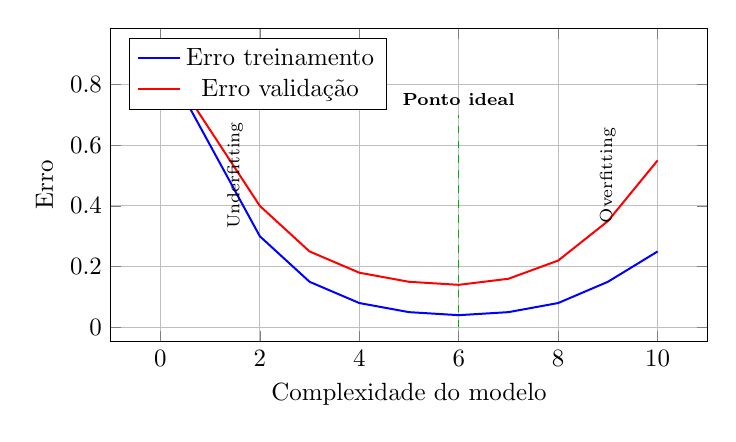
\begin{tikzpicture}[scale=0.9]
\begin{axis}[xlabel={Complexidade do modelo},
ylabel={Erro},
legend pos=north west,
width=10cm, height=6cm,
grid=major
]
\addplot[blue, thick] coordinates {
(0, 0.9) (1, 0.6) (2, 0.3) (3, 0.15) (4, 0.08)
(5, 0.05) (6, 0.04) (7, 0.05) (8, 0.08) (9, 0.15)
(10, 0.25)
};
\addlegendentry{Erro treinamento}
\addplot[red, thick] coordinates {
(0, 0.9) (1, 0.65) (2, 0.4) (3, 0.25) (4, 0.18)
(5, 0.15) (6, 0.14) (7, 0.16) (8, 0.22) (9, 0.35)
(10, 0.55)
};
\addlegendentry{Erro validação}
\draw[dashed, green!70!black] (axis cs:6,0) -- (axis cs:6,0.7);
\node at (axis cs:6,0.75) {\scriptsize\textbf{Ponto ideal}};
\node[rotate=90] at (axis cs:1.5,0.5) {\scriptsize Underfitting};
\node[rotate=90] at (axis cs:9,0.5) {\scriptsize Overfitting};
\end{axis}
\end{tikzpicture}
\end{figure}
\subsection{Aplicação: Classificação de Intenções em Agentes}
No \opencodeeco{}, o Behavioral Gate (SPEC-038) utiliza um classificador
supervisionado para categorizar intenções de agentes em quatro categorias:
segura, moderada, arriscada e bloqueada \cite{opencode2026spec038}.
\begin{lstlisting}[style=pythonstyle]
from sklearn.ensemble import RandomForestClassifier
from sklearn.model_selection import cross_val_score
# Pipeline de classificacao de intencoes
class IntentionClassifier:
def __init__(self):
self.model = RandomForestClassifier(n_estimators=200, max_depth=8)
self.features = ["trust_score", "action_risk", "history_violations",
"resource_sensitivity", "compliance_score"
]
def extract_features(self, action, context):
return [[context.get("trust_score", 0.5),
1.0 if action in RISKY_ACTIONS else 0.0,
context.get("violations", 0),
context.get("resource_level", 0.5),
context.get("compliance", 1.0)
]]
def train(self, X, y):
scores = cross_val_score(self.model, X, y, cv=5)
print(f"Acuracia CV: {scores.mean():.3f} +/- {scores.std():.3f}")
self.model.fit(X, y)
def classify(self, action, context):
X = self.extract_features(action, context)
proba = self.model.predict_proba(X)[0]
return {
"categoria": self.model.classes_[np.argmax(proba)],
"confianca": np.max(proba),
"threshold_excedido": np.max(proba) > 0.7
}
\end{lstlisting}
\subsection{Exercícios — Aprendizado de Máquina}
\begin{exercicio}[Nivel Básico]
Implemente a regressão linear usando gradiente descendente em vez da solução
analítica. Compare a convergência para diferentes taxas de aprendizado.
\end{exercicio}
\begin{exercicio}[Nivel Básico]
Explique a diferença entre underfitting e overfitting. Desenhe (conceitualmente)
como cada um se manifesta em uma curva de aprendizado.
\end{exercicio}
\begin{exercicio}[Nivel Intermediário]
Usando o \texttt{make\_classification} (do \\\hspace*{2em}\texttt{sklearn.datasets}), compare a acurácia
de SVM, Random Forest e k-NN em validação cruzada 5-fold. Qual generaliza
melhor? Por quê?
\end{exercicio}
\begin{exercicio}[Nivel Intermediário]
Implemente o algoritmo k-means do zero e teste-o no dataset Iris. Compare
seus resultados com o \texttt{sklearn.cluster.KMeans}.
\end{exercicio}
\begin{exercicio}[Nivel Avançado]
Projete um classificador de intenções para o Behavioral Gate do
\opencodeeco{} que utilize regularização L2 e validação cruzada para
selecionar hiperparâmetros automaticamente.
\end{exercicio}
% =============================================================================
% SEÇÃO 2.3: REDES NEURAIS E DEEP LEARNING
% Nível: Intermediário (~12 laudas)
% =============================================================================
\section{Redes Neurais e Deep Learning}
\label{sec:redes-neurais}
\nivelintermediario

\paragraph{Inspiração biológica, execução matemática.} Se o aprendizado de
máquina tradicional usa algoritmos projetados à mão, o \textit{deep learning}
constrói suas próprias representações --- camada por camada. Cada camada
extrai características progressivamente mais abstratas: da borda ao olho, do
olho ao rosto, do rosto à pessoa. No \opencodeeco{}, o deep learning está
na base dos LLMs que alimentam os agentes, nos modelos de embedding que
medem similaridade entre skills e nos classificadores do Behavioral Gate.

As redes neurais artificiais são modelos computacionais inspirados na
estrutura do cérebro biológico. O \destaque{Deep Learning} refere-se a
redes neurais com múltiplas camadas ocultas, capazes de aprender
representações hierárquicas complexas \cite{goodfellow2016deep,
lecun2015deep}.
\subsection{O Neurônio Artificial}
\begin{definicao}[Neurônio Artificial de McCulloch-Pitts]
O primeiro modelo matemático de um neurônio foi proposto por McCulloch e
Pitts em 1943 \cite{mcculloch1943logical}. Ele recebe entradas binárias
$x_1, \ldots, x_n$, cada uma multiplicada por um peso $w_i$, e produz uma
saída:
\[y = \phi\left(\sum_{i=1}^n w_i x_i + b\right)
\]
onde $\phi$ é a função de ativação.
\end{definicao}
\subsection{Perceptron}
O \destaque{Perceptron} de Rosenblatt \cite{rosenblatt1958perceptron} foi
o primeiro algoritmo de aprendizado para redes neurais:
\[y = \begin{cases}
1 & \text{se } \sum w_i x_i + b > 0 \\
0 & \text{caso contrário}
\end{cases}
\]
\begin{lstlisting}[style=pythonstyle]
class Perceptron:
def __init__(self, n_features, lr=0.01):
self.w = np.zeros(n_features)
self.b = 0.0
self.lr = lr
def predict(self, X):
return np.where(X @ self.w + self.b > 0, 1, 0)
def train(self, X, y, epochs=100):
for _ in range(epochs):
for xi, yi in zip(X, y):
y_pred = self.predict(xi)
erro = yi - y_pred
self.w += self.lr * erro * xi
self.b += self.lr * erro
\end{lstlisting}
\subsection{Multilayer Perceptron (MLP) e Backpropagation}
O MLP estende o Perceptron com uma ou mais \destaque{camadas ocultas}
entre a entrada e a saída \cite{rumelhart1986learning}.
\begin{definicao}[MLP]
Uma rede MLP com $L$ camadas é definida recursivamente:
\begin{align*}
h^{(0)} &= x \\
z^{(l)} &= W^{(l)} h^{(l-1)} + b^{(l)} \\
h^{(l)} &= \phi^{(l)}(z^{(l)}) \quad \text{para } l = 1, \ldots, L \\
\hat{y} &= h^{(L)}
\end{align*}
onde $W^{(l)}$, $b^{(l)}$ são os parâmetros da camada $l$ e $\phi^{(l)}$ é
a função de ativação \cite{goodfellow2016deep}.
\end{definicao}
O treinamento usa \destaque{backpropagation}: o gradiente do erro é
propagado da saída para a entrada aplicando a regra da cadeia:
\[\frac{\partial \mathcal{L}}{\partial W^{(l)}} =
\frac{\partial \mathcal{L}}{\partial h^{(L)}} \cdot
\frac{\partial h^{(L)}}{\partial z^{(L)}} \cdot
\frac{\partial z^{(L)}}{\partial h^{(L-1)}} \cdots
\frac{\partial h^{(l)}}{\partial z^{(l)}} \cdot
\frac{\partial z^{(l)}}{\partial W^{(l)}}
\]
\begin{lstlisting}[style=pythonstyle]
class MLP:
def __init__(self, camadas: list):
"""camadas = [entrada, oculta1,..., saida]"""
self.params = {}
for i in range(1, len(camadas)):
self.params[f"W{i}"] = np.random.randn(camadas[i-1], camadas[i]) * 0.01
self.params[f"b{i}"] = np.zeros(camadas[i])
self.n_camadas = len(camadas) - 1
def forward(self, X):
self.cache = {"A0": X}
for i in range(1, self.n_camadas + 1):
Z = self.cache[f"A{i-1}"] @ self.params[f"W{i}"] \
+ self.params[f"b{i}"]
A = np.maximum(Z, 0) # ReLU
self.cache[f"Z{i}"] = Z
self.cache[f"A{i}"] = A
return self.cache[f"A{self.n_camadas}"]
def backward(self, X, y, output):
m = X.shape[0]
dA = output - y # derivada MSE
for i in range(self.n_camadas, 0, -1):
dZ = dA * (self.cache[f"Z{i}"] > 0) # ReLU deriv
dW = (1/m) * self.cache[f"A{i-1}"].T @ dZ
db = (1/m) * np.sum(dZ, axis=0)
dA = dZ @ self.params[f"W{i}"].T
self.params[f"W{i}"] -= 0.01 * dW
self.params[f"b{i}"] -= 0.01 * db
\end{lstlisting}
\subsection{Funções de Ativação}
A Tabela~\ref{tab:ativacoes} apresenta as principais funções de ativação.
\begin{table}[htb]
\centering
    \small
\caption{Funções de ativação mais comuns}
\label{tab:ativacoes}
    \resizebox{\textwidth}{!}{
\begin{tabular}{lll}
\toprule
\textbf{Função} & \textbf{Fórmula} & \textbf{Característica} \\
\midrule
Sigmoid & $\sigma(z) = \frac{1}{1+e^{-z}}$ & Saída em $(0,1)$, desvanece \\
Tanh & $\tanh(z) = \frac{e^z - e^{-z}}{e^z + e^{-z}}$ & Saída em $(-1,1)$ \\
ReLU & $\text{ReLU}(z) = \max(0, z)$ & Não satura, neurônios mortos \\
GELU & $\text{GELU}(z) = z\Phi(z)$ & Suave, usada em transformers \\
\bottomrule
\end{tabular}
    }
\end{table}
A função \destaque{ReLU} (\textit{Rectified Linear Unit}) é a mais utilizada
em redes profundas por mitigar o problema do gradiente evanescente
\cite{nair2010relu}. A \destaque{GELU} (\textit{Gaussian Error Linear Unit})
é preferida em modelos Transformer modernos por sua curva suave que preserva
gradientes \cite{hendrycks2016gaussian}.
\subsection{Redes Convolucionais (CNNs)}
As CNNs são especializadas em processamento de dados com estrutura de grade,
como imagens \cite{lecun1998gradient, krizhevsky2012imagenet}. Suas camadas
principais são:
\begin{itemize}
\item \destaque{Convolução}: aplica filtros (kernels) que deslizam sobre a
entrada, detectando padrões locais como bordas e texturas.
\item \destaque{Pooling}: reduz a dimensionalidade espacial (ex.:
max-pooling $2\times2$ mantém o maior valor em cada janela).
\item \destaque{Fully Connected}: camada densa que combina as
características extraídas para a classificação final.
\end{itemize}
\begin{figure}[htb]
\centering
\caption{Arquitetura de uma CNN para classificação de imagens}
\label{fig:cnn}
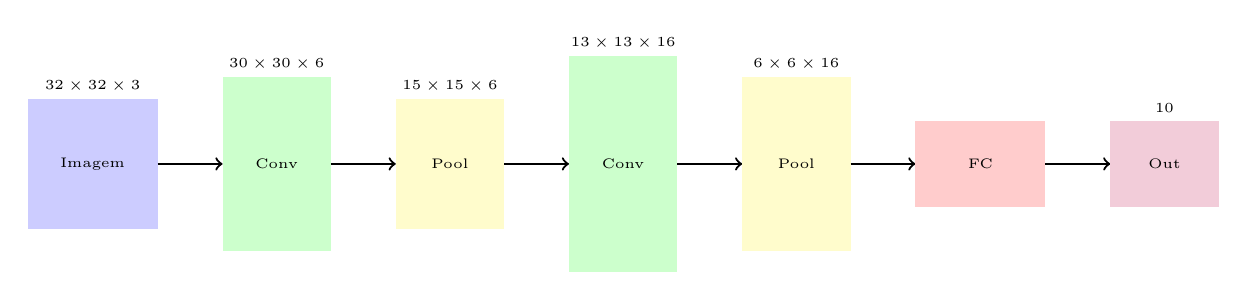
\begin{tikzpicture}[scale=0.55]
\fill[blue!20] (0, -1) rectangle (3, 2);
\node at (1.5, 0.5) {\tiny Imagem};
\node at (1.5, 2.3) {\tiny $32\times32\times3$};
\draw[->, thick] (3, 0.5) -- (4.5, 0.5);
\fill[green!20] (4.5, -1.5) rectangle (7, 2.5);
\node at (5.75, 0.5) {\tiny Conv};
\node at (5.75, 2.8) {\tiny $30\times30\times6$};
\draw[->, thick] (7, 0.5) -- (8.5, 0.5);
\fill[yellow!20] (8.5, -1) rectangle (11, 2);
\node at (9.75, 0.5) {\tiny Pool};
\node at (9.75, 2.3) {\tiny $15\times15\times6$};
\draw[->, thick] (11, 0.5) -- (12.5, 0.5);
\fill[green!20] (12.5, -2) rectangle (15, 3);
\node at (13.75, 0.5) {\tiny Conv};
\node at (13.75, 3.3) {\tiny $13\times13\times16$};
\draw[->, thick] (15, 0.5) -- (16.5, 0.5);
\fill[yellow!20] (16.5, -1.5) rectangle (19, 2.5);
\node at (17.75, 0.5) {\tiny Pool};
\node at (17.75, 2.8) {\tiny $6\times6\times16$};
\draw[->, thick] (19, 0.5) -- (20.5, 0.5);
\fill[red!20] (20.5, -0.5) rectangle (23.5, 1.5);
\node at (22, 0.5) {\tiny FC};
\draw[->, thick] (23.5, 0.5) -- (25, 0.5);
\fill[purple!20] (25, -0.5) rectangle (27.5, 1.5);
\node at (26.25, 0.5) {\tiny Out};
\node at (26.25, 1.8) {\tiny $10$};
\end{tikzpicture}
\end{figure}
\subsection{Redes Recorrentes (RNNs e LSTMs)}
RNNs processam sequências mantendo um estado oculto que captura informação
de passos anteriores \cite{goodfellow2016deep}:
\[h_t = \phi(W_{hh} h_{t-1} + W_{xh} x_t + b_h)
\]
As \destaque{LSTMs} (\textit{Long Short-Term Memory}) resolvem o problema do
desvanecimento do gradiente introduzindo um mecanismo de portas que controla
o fluxo de informação \cite{hochreiter1997long}:
\begin{align*}
f_t &= \sigma(W_f [h_{t-1}, x_t] + b_f) \quad \text{(porta de esquecimento)} \\
i_t &= \sigma(W_i [h_{t-1}, x_t] + b_i) \quad \text{(porta de entrada)} \\
\tilde{C}_t &= \tanh(W_C [h_{t-1}, x_t] + b_C) \quad \text{(candidato)} \\
C_t &= f_t \odot C_{t-1} + i_t \odot \tilde{C}_t \quad \text{(célula)} \\
o_t &= \sigma(W_o [h_{t-1}, x_t] + b_o) \quad \text{(porta de saída)} \\
h_t &= o_t \odot \tanh(C_t)
\end{align*}
\begin{lstlisting}[style=pythonstyle]
class LSTMCell:
def __init__(self, input_dim, hidden_dim):
self.hidden_dim = hidden_dim
# Inicializacao dos pesos das 4 portas
self.Wf = np.random.randn(input_dim + hidden_dim, hidden_dim) * 0.01
self.Wi = np.random.randn(input_dim + hidden_dim, hidden_dim) * 0.01
self.Wc = np.random.randn(input_dim + hidden_dim, hidden_dim) * 0.01
self.Wo = np.random.randn(input_dim + hidden_dim, hidden_dim) * 0.01
self.bf = np.zeros(hidden_dim)
self.bi = np.zeros(hidden_dim)
self.bc = np.zeros(hidden_dim)
self.bo = np.zeros(hidden_dim)
def forward(self, x, h_prev, c_prev):
concat = np.concatenate([h_prev, x])
f = 1 / (1 + np.exp(-(concat @ self.Wf + self.bf)))
i = 1 / (1 + np.exp(-(concat @ self.Wi + self.bi)))
c_candidate = np.tanh(concat @ self.Wc + self.bc)
c = f * c_prev + i * c_candidate
o = 1 / (1 + np.exp(-(concat @ self.Wo + self.bo)))
h = o * np.tanh(c)
return h, c
\end{lstlisting}
\subsection{Regularização em Redes Profundas}
\subsubsection{Dropout}
\begin{definicao}[Dropout]
Durante o treinamento, neurônios são ``desligados'' aleatoriamente com
probabilidade $p$, forçando a rede a aprender representações redundantes e
reduzindo overfitting \cite{srivastava2014dropout}.
\end{definicao}
\[h_{\text{drop}} = h \odot m, \quad m_i \sim \text{Bernoulli}(1-p)
\]
\subsubsection{Batch Normalization}
\begin{definicao}[Batch Normalization]
Normaliza a saída de cada camada para ter média zero e variância unitária,
estabilizando o treinamento e permitindo taxas de aprendizado mais altas
\cite{ioffe2015batch}.
\end{definicao}
\[\hat{x}^{(k)} = \frac{x^{(k)} - \mu_B}{\sqrt{\sigma_B^2 + \epsilon}}, \quad
y^{(k)} = \gamma^{(k)} \hat{x}^{(k)} + \beta^{(k)}
\]
\subsection{Aplicação: Feature Extraction em Pipelines de Agentes}
No \opencodeeco{}, redes neurais são usadas como extratores de
características em pipelines multiagentes. Por exemplo, o módulo de
análise semântica utiliza embeddings gerados por redes pré-treinadas para
representar intenções de agentes \cite{opencode2026ecosystem}:
\begin{lstlisting}[style=pythonstyle]
# Extrator de caracteristicas neurais para agentes
class NeuralFeatureExtractor:
def __init__(self, input_dim=100, hidden_dim=64):
self.W1 = np.random.randn(input_dim, hidden_dim) * 0.01
self.b1 = np.zeros(hidden_dim)
def relu(self, z):
return np.maximum(0, z)
def extract(self, x: np.ndarray) -> np.ndarray:
"""Converte entrada bruta em embedding de caracteristicas."""
h = self.relu(x @ self.W1 + self.b1)
# Normalizacao L2
norm = np.linalg.norm(h, keepdims=True) + 1e-8
return h / norm
def similarity(self, emb1, emb2):
return float(emb1 @ emb2.T) # cosseno
# Uso: comparar intencoes de dois agentes
extractor = NeuralFeatureExtractor()
intencao_a = np.random.randn(100)
intencao_b = np.random.randn(100)
sim = extractor.similarity(extractor.extract(intencao_a),
extractor.extract(intencao_b))
print(f"Similaridade entre intencoes: {sim:.3f}")
\end{lstlisting}
\subsection{Exercícios — Redes Neurais}
\begin{exercicio}[Nivel Básico]
Implemente um Perceptron para a porta lógica XOR. Explique por que um único
Perceptron não consegue resolver este problema.
\end{exercicio}
\begin{exercicio}[Nivel Intermediário]
Implemente uma MLP com uma camada oculta para classificar o dataset
\texttt{make\_moons} do sklearn. Varie o número de neurônios na camada oculta
e observe o efeito na fronteira de decisão.
\end{exercicio}
\begin{exercicio}[Nivel Intermediário]
Compare o desempenho de ReLU, sigmoid e tanh em uma MLP com 3 camadas
ocultas treinada no dataset MNIST. Qual ativação converge mais rápido?
\end{exercicio}
\begin{exercicio}[Nivel Avançado]
Implemente uma CNN simples (2 camadas convolucionais + 2 camadas totalmente
conectadas) do zero usando apenas NumPy. Teste no dataset CIFAR-10.
\end{exercicio}
\begin{exercicio}[Nivel Avançado]
Usando o \opencodeeco{} como referência, projete um pipeline de feature
extraction que utilize uma LSTM para processar sequências de ações de agentes
e classificar padrões de comportamento.
\end{exercicio}
% =============================================================================
% SEÇÃO 2.4: TRANSFORMERS E LLMs
% Nível: Avançado (~12 laudas)
% =============================================================================
\section{Transformers e Modelos de Linguagem de Grande Escala}
\label{sec:transformers-llms}
\nivelavancado

\paragraph{A revolução da atenção.} Até 2017, redes neurais processavam
sequências de forma sequencial (uma palavra de cada vez) com LSTMs e GRUs.
O Transformer mudou tudo: ele processa todas as palavras em paralelo,
usando um mecanismo de \textbf{atenção} que decide quais partes da entrada
são relevantes para cada posição da saída. É como ler um livro inteiro de
uma só vez, em vez de palavra por palavra. No \opencodeeco{}, os 128 agentes
utilizam LLMs baseados em Transformers (DeepSeek, GPT, Claude) como motor
de raciocínio, combinados com o mecanismo de atenção para selecionar MCPs e
skills relevantes em cada contexto.

A publicação do artigo \textit{Attention Is All You Need} por Vaswani et
al. \cite{vaswani2017attention} em 2017 revolucionou o processamento de
linguagem natural e, subsequentemente, toda a inteligência artificial.
A arquitetura Transformer eliminou a necessidade de recorrência e convolução,
substituindo-as por mecanismos de atenção que permitem processamento
paralelo e captura de dependências de longo alcance.
\subsection{A Arquitetura Transformer}
O Transformer segue uma estrutura \destaque{encoder-decoder}. O encoder
mapeia a sequência de entrada em representações contínuas; o decoder gera
a sequência de saída a partir dessas representações.
\begin{figure}[htb]
\centering
\caption{Arquitetura Transformer (adaptado de Vaswani et al., 2017)}
\label{fig:transformer}
\begin{tikzpicture}[scale=0.8, transform shape]
\tikzstyle{block} = [rectangle, draw, fill=blue!10,
text centered, minimum height=1.5em, minimum width=4em]
\tikzstyle{block2} = [rectangle, draw, fill=green!10,
text centered, minimum height=1.5em, minimum width=4em]
\node[block] (inp) {Entrada};
\node[block, above=of inp] (emb) {Embedding};
\node[block, above=of emb] (pe) {Pos. Encoding};
\node[block2, above=of pe] (attn) {Multi-Head Attention};
\node[block2, above=of attn] (add1) {Add \& Norm};
\node[block2, above=of add1] (ffn) {Feed Forward};
\node[block2, above=of ffn] (add2) {Add \& Norm};
\node[block, above=of add2] (out_enc) {Encoder $\times N$};
\node[block, right=6cm of inp] (inp2) {Saída};
\node[block, above=of inp2] (emb2) {Embedding};
\node[block, above=of emb2] (pe2) {Pos. Encoding};
\node[block2, above=of pe2] (attn2) {Masked MHA};
\node[block2, above=of attn2] (add3) {Add \& Norm};
\node[block2, above=of add3] (attn3) {Cross-Attention};
\node[block2, above=of attn3] (add4) {Add \& Norm};
\node[block2, above=of add4] (ffn2) {Feed Forward};
\node[block2, above=of ffn2] (add5) {Add \& Norm};
\node[block, above=of add5] (out_dec) {Decoder $\times N$};
\node[block, above=of out_dec] (linear) {Linear};
\node[block, above=of linear] (softmax) {Softmax};
\draw[->] (inp) -- (emb);
\draw[->] (emb) -- (pe);
\draw[->] (pe) -- (attn);
\draw[->] (attn) -- (add1);
\draw[->] (add1) -- (ffn);
\draw[->] (ffn) -- (add2);
\draw[->] (add2) -- (out_enc);
\draw[->] (inp2) -- (emb2);
\draw[->] (emb2) -- (pe2);
\draw[->] (pe2) -- (attn2);
\draw[->] (attn2) -- (add3);
\draw[->] (add3) -- (attn3);
\draw[->] (add3.east) -- ++(0.5,0) |- (attn3.east);
\draw[->] (attn3) -- (add4);
\draw[->] (add4) -- (ffn2);
\draw[->] (ffn2) -- (add5);
\draw[->] (add5) -- (out_dec);
\draw[->] (out_dec) -- (linear);
\draw[->] (linear) -- (softmax);
\draw[->, dashed] (out_enc.east) -- ++(1,0) |- (attn3.east);
\draw[->, dashed] (out_enc.east) -- ++(1,0) |- (add4.east);
\node[below=0.2cm of out_enc] {\scriptsize Codificador};
\node[below=0.2cm of out_dec] {\scriptsize Decodificador};
\end{tikzpicture}
\end{figure}
\subsection{Mecanismo de Atenção}
O mecanismo de atenção é o coração do Transformer.
\begin{definicao}[Atenção por Produto Escalar]
Dados uma consulta $Q$, chave $K$ e valor $V$, a atenção é computada como:
\[\text{Attention}(Q, K, V) = \text{softmax}\left(\frac{QK^\top}{\sqrt{d_k}}\right)V
\]
onde $d_k$ é a dimensão das chaves, e o fator $\sqrt{d_k}$ evita que os
produtos escalares cresçam excessivamente \cite{vaswani2017attention}.
\end{definicao}
\begin{definicao}[Multi-Head Attention]
Em vez de uma única função de atenção, o Transformer projeta $Q$, $K$, $V$
$h$ vezes com diferentes matrizes de peso lineares, permitindo que o modelo
atente a informações de diferentes subespaços representacionais
\cite{vaswani2017attention}:
\begin{align*}
\text{MultiHead}(Q, K, V) &= \text{Concat}(\text{head}_1, \ldots, \text{head}_h) W^O \\
\text{head}_i &= \text{Attention}(Q W_i^Q, K W_i^K, V W_i^V)
\end{align*}
\end{definicao}
A Figura~\ref{fig:attention} ilustra visualmente o mecanismo.
\begin{figure}[htb]
\centering
\caption{Mecanismo de atenção: consulta, chave, valor e saída ponderada}
\label{fig:attention}
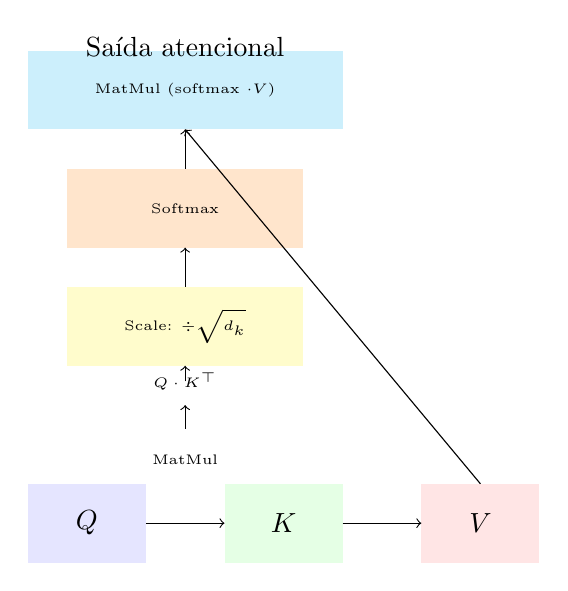
\begin{tikzpicture}[scale=1.0]
\fill[blue!10] (0, 0) rectangle (1.5, 1);
\node at (0.75, 0.5) {$Q$};
\fill[green!10] (2.5, 0) rectangle (4, 1);
\node at (3.25, 0.5) {$K$};
\fill[red!10] (5, 0) rectangle (6.5, 1);
\node at (5.75, 0.5) {$V$};
\draw[->] (1.5, 0.5) -- (2.5, 0.5);
\draw[->] (4, 0.5) -- (5, 0.5);
\node at (2, 1.3) {\tiny MatMul};
\node at (2, 2.3) {\tiny $Q \cdot K^\top$};
\draw[->] (2, 1.7) -- (2, 2.0);
\fill[yellow!20] (0.5, 2.5) rectangle (3.5, 3.5);
\node at (2, 3.0) {\tiny Scale: $\div \sqrt{d_k}$};
\draw[->] (2, 2.3) -- (2, 2.5);
\fill[orange!20] (0.5, 4.0) rectangle (3.5, 5.0);
\node at (2, 4.5) {\tiny Softmax};
\draw[->] (2, 3.5) -- (2, 4.0);
\fill[cyan!20] (0, 5.5) rectangle (4, 6.5);
\node at (2, 6.0) {\tiny MatMul (softmax $\cdot V$)};
\draw[->] (2, 5.0) -- (2, 5.5);
\draw[->] (5.75, 1.0) -- (2, 5.5);
\node[below] at (2, 6.8) {Saída atencional};
\end{tikzpicture}
\end{figure}
\subsection{Positional Encoding e Layer Normalization}
Como o Transformer não possui recorrência ou convolução, ele precisa de
informação posicional. Vaswani et al. \cite{vaswani2017attention} usam
codificação senoidal:
\begin{align*}
PE_{(pos, 2i)} &= \sin\left(\frac{pos}{10000^{2i/d_{\text{model}}}}\right) \\
PE_{(pos, 2i+1)} &= \cos\left(\frac{pos}{10000^{2i/d_{\text{model}}}}\right)
\end{align*}
Alternativas modernas incluem \destaque{RoPE} (\textit{Rotary Position
Embedding}), usada em modelos como Llama e DeepSeek, que codifica posição
através de rotações no espaço de embedding \cite{su2024roformer}.
A \destaque{layer normalization} \cite{ba2016layer} normaliza as ativações
através das características (não do batch, como batch normalization):
\[\mu = \frac{1}{H} \sum_{i=1}^H a_i, \quad
\sigma^2 = \frac{1}{H} \sum_{i=1}^H (a_i - \mu)^2, \quad
\text{LayerNorm}(a) = \frac{a - \mu}{\sqrt{\sigma^2 + \epsilon}} \odot \gamma + \beta
\]
\subsection{Modelos Pré-Treinados: BERT, GPT, Llama, DeepSeek}
A arquitetura Transformer deu origem a duas famílias principais de modelos
pré-treinados:
\subsubsection*{BERT (Bidirectional Encoder Representations from Transformers)}
BERT \cite{devlin2019bert} utiliza apenas o encoder do Transformer e é
treinado com duas tarefas: \textit{masked language modeling} (prever
palavras mascaradas) e \textit{next sentence prediction}. É ideal para
tarefas de compreensão como classificação de texto e resposta a perguntas.
\subsubsection*{GPT (Generative Pre-trained Transformer)}
GPT \cite{radford2018gpt} utiliza apenas o decoder do Transformer e é
treinado para predizer a próxima palavra (\textit{language modeling}
autoregressivo). O GPT-3 \cite{brown2020language} demonstrou que aumentar a
escala (175 bilhões de parâmetros) produz aprendizado \textit{few-shot}
emergente. O GPT-4 \cite{achiam2023gpt4} adicionou raciocínio multimodal e
instrução refinada.
\subsubsection*{Llama}
Llama \cite{touvron2023llama} é uma família de modelos abertos da Meta que
demonstrou que modelos menores (7B, 13B, 70B) podem competir com modelos
maiores quando treinados com mais dados. Llama utiliza RoPE e
pré-normalização.
\subsubsection*{DeepSeek}
DeepSeek-V2 \cite{deepseek2024deepseek} introduziu inovações como
\textit{Multi-head Latent Attention} (MLA) e \textit{DeepSeekMoE} (arquitetura
Mixture-of-Experts), alcançando eficiência comparável a GPT-4 com custo
computacional significativamente menor. O \opencodeeco{} utiliza
deepseek-v4-pro como modelo padrão para operações de raciocínio e geração
de código.
\subsection{RLHF, Instruction Tuning e Chain-of-Thought}
\subsubsection*{Instruction Tuning}
O ajuste por instruções (\textit{instruction tuning}) refina modelos
pré-treinados em conjuntos de dados de instruções, melhorando a capacidade
de seguir comandos \cite{chung2022scaling}.
\subsubsection*{RLHF (Reinforcement Learning from Human Feedback)}
RLHF \cite{ouyang2022training} alinha modelos a preferências humanas através
de três estágios:
\begin{enumerate}
\item \textbf{Supervised Fine-Tuning} (SFT): ajuste supervisionado em
demonstrações humanas.
\item \textbf{Reward Modeling}: treina um modelo de recompensa para
classificar saídas preferidas.
\item \textbf{PPO Optimization}: otimiza a política usando o modelo de
recompensa como sinal.
\end{enumerate}
\subsubsection*{Chain-of-Thought (CoT)}
O raciocínio \textit{chain-of-thought} \cite{wei2022chain} elicia
raciocínio passo a passo em LLMs, melhorando significativamente o
desempenho em tarefas que exigem múltiplas inferências:
\begin{lstlisting}[style=pythonstyle]
# Exemplo: Chain-of-Thought no OpenCode CLI
prompt = """
Pergunta: Se um agente tem trust_score=0.6,
action_risk=0.8, e esta em shadow_mode=False,
o Behavioral Gate deve permitir a acao?
Raciocinio passo a passo:
1. Trust score (0.6) esta abaixo do threshold (0.7)
2. Acao tem risco alto (0.8 > 0.5)
3. nao esta em shadow mode
4. Regra: trust < 0.7 E risk > 0.5 -> BLOQUEAR
5. Portanto, a acao deve ser BLOQUEADA
Resposta: BLOQUEAR
"""
\end{lstlisting}
\subsection{Aplicação: OpenCode CLI com DeepSeek-V4-Pro}
O \opencodeeco{} integra deepseek-v4-pro como motor de raciocínio padrão.
A CLI utiliza o modelo para interpretar comandos, gerar código e coordenar
agentes \cite{opencode2026ecosystem}:
\begin{lstlisting}[style=pythonstyle]
# Configuracao do modelo no OpenCode CLI
MODEL_CONFIG = {
"model": "deepseek-v4-pro",
"context_window": 200_000, # 200K tokens
"max_output": 128_000, # 128K tokens de saida
"supports_vision": False,
"cost_per_1k_input": 0.0001, # USD (gratuito)
"cost_per_1k_output": 0.0001, # USD (gratuito)
"specialties": ["raciocinio_cadeia", "geracao_codigo",
"analise_tecnica", "matematica_simbolica"
]
}
class OpenCodeLLMInterface:
"""Interface entre o ecossistema e o LLM."""
def __init__(self, config: dict):
self.config = config
self.conversation_history = []
def generate(self, prompt: str,
max_tokens: int = 4096) -> str:
"""Gera resposta usando Chain-of-Thought."""
system = ("voce e um assistente de engenharia de "
"software especializado em agentes cognitivos. "
"Responda em portugues do Brasil formal.")
messages = [{"role": "system", "content": system},
*self.conversation_history[-10:],
{"role": "user", "content": prompt}
]
# Simulacao da chamada a API
response = self._call_llm_api(messages)
self.conversation_history.append({"role": "user", "content": prompt})
self.conversation_history.append({"role": "assistant", "content": response})
return response
def _call_llm_api(self, messages: list) -> str:
"""Placeholder para chamada real a API DeepSeek."""
return "Resposta simulada do deepseek-v4-pro."
\end{lstlisting}
\subsection{Exercícios — Transformers e LLMs}
\begin{exercicio}[Nivel Intermediário]
Implemente a função de atenção por produto escalar (scaled dot-product
attention) do zero usando NumPy. Teste com $Q, K, V$ de dimensões
$4 \times 8$.
\end{exercicio}
\begin{exercicio}[Nivel Intermediário]
Explique por que o positional encoding senoidal permite que o Transformer
generalize para sequências mais longas do que as vistas no treinamento.
\end{exercicio}
\begin{exercicio}[Nivel Avançado]
Implemente uma camada Multi-Head Attention com 2 cabeças de atenção.
Compare o gradiente da atenção com e sem o fator de escala $\sqrt{d_k}$.
\end{exercicio}
\begin{exercicio}[Nivel Avançado]
Usando a API do \texttt{transformers} (Hugging Face), carregue um modelo
BERT e extraia embeddings para a frase ``O OpenCode possui 128 agentes
cognitivos''. Visualize os pesos de atenção.
\end{exercicio}
\begin{exercicio}[Nivel Avançado]
Crie um prompt chain-of-thought para o deepseek-v4-pro que resolva o
problema: ``Dado trust\_score=0.4, violations=3, shadow\_mode=True, o
Behavioral Gate deve permitir a ação?''.
\end{exercicio}
% =============================================================================
% SEÇÃO 2.5: ENGENHARIA DE PROMPTS E RACIOCÍNIO
% Nível: Avançado (~8 laudas)
% =============================================================================
\section{Engenharia de Prompts e Raciocínio}
\label{sec:engenharia-prompts}
\nivelavancado

\paragraph{Programar com linguagem natural.} Se um Transformer é o motor, o
prompt é o volante. A engenharia de prompts é a arte e a ciência de
formular instruções para LLMs de modo a obter respostas úteis, precisas e
seguras. Não se trata de adivinhação: técnicas como \textit{chain-of-thought}
(``pense passo a passo''), \textit{few-shot} (fornecer exemplos) e
\textit{role prompting} (atribuir uma persona) têm base teórica e resultados
mensuráveis. No \opencodeeco{}, cada um dos 128 agentes possui um prompt
sistêmico projectado para maximizar sua especialidade --- e o Trust Engine
monitora se os agentes estão seguindo o prompt ou desviando do objetivo.

A engenharia de prompts emergiu como uma disciplina crucial para extrair
raciocínio de alta qualidade de LLMs. Diferentemente da programação
tradicional, onde instruções são executadas deterministicamente, prompts
são ``programas em linguagem natural'' cuja execução depende da
interpretação probabilística do modelo \cite{white2023prompt}.
\subsection{Zero-Shot e Few-Shot Prompting}
\begin{definicao}[Zero-Shot Prompting]
O modelo realiza a tarefa sem exemplos prévios. Apenas a instrução é
fornecida \cite{brown2020language}.
\end{definicao}
\begin{definicao}[Few-Shot Prompting]
O modelo recebe $k$ exemplos completos (entrada + saída) antes de ser
solicitado a responder um novo caso \cite{brown2020language}.
\end{definicao}
\begin{lstlisting}[style=pythonstyle]
# Zero-shot: sem exemplos
zero_shot = """
Classifique a intencao do agente como
SEGURA, MODERADA ou ARRISCADA:
trust_score=0.8, action='read_file'
"""
# Few-shot: com 2 exemplos
few_shot = """
Classifique a intencao do agente:
trust_score=0.9, action='list_dir' -> SEGURA
trust_score=0.3, action='delete_file' -> ARRISCADA
trust_score=0.6, action='modify_config' ->
"""
\end{lstlisting}
\subsection{Chain-of-Thought (Wei et al., 2022)}
CoT \cite{wei2022chain} elicia raciocínio passo a passo, melhorando o
desempenho em tarefas aritméticas, lógicas e simbólicas:
\begin{lstlisting}[style=pythonstyle]
prompt_cot = """
Pergunta: Se o TrustScorer usa blend 70/30,
e o score objetivo e 0.6 e o score subjetivo e 0.8,
qual e o trust_score final?
Raciocinio passo a passo:
1. Blend = 0.7 * score_objetivo + 0.3 * score_subjetivo
2. Blend = 0.7 * 0.6 + 0.3 * 0.8
3. Blend = 0.42 + 0.24
4. Blend = 0.66
5. Trust score = 0.66
Resposta: 0.66
"""
\end{lstlisting}
\subsection{Self-Consistency (Wang et al., 2023)}
\begin{definicao}[Self-Consistency]
Em vez de seguir um único caminho de raciocínio, amostram-se múltiplos
caminhos ($N \geq 5$) e a resposta final é determinada por votação
majoritária \cite{wang2023selfconsistency}.
\end{definicao}
\[\hat{y} = \arg\max_y \sum_{i=1}^N \mathds{1}[f_i(x) = y]
\]
onde $f_i(x)$ é a resposta do $i$-ésimo caminho de raciocínio.
\begin{lstlisting}[style=pythonstyle]
class SelfConsistency:
def __init__(self, n_paths=5):
self.n_paths = n_paths
def solve(self, prompt: str, llm_fn) -> str:
"""Amostra multiplos caminhos e retorna o mais consistente."""
respostas = []
for _ in range(self.n_paths):
resposta = llm_fn(prompt + "\nRaciocinio:")
respostas.append(resposta)
from collections import Counter
votacao = Counter(respostas)
return votacao.most_common(1)[0][0]
\end{lstlisting}
\subsection{ReAct: Raciocínio + Ação (Yao et al., 2023)}
ReAct \cite{yao2023react} intercala raciocínio (\textit{reasoning}) com
ação (\textit{acting}), permitindo que o agente busque informações externas
e atualize seu raciocínio:
\[\text{Ciclo ReAct: } \text{Pensar} \to \text{Agir} \to \text{Observar} \to \text{Pensar} \to \ldots
\]
\begin{lstlisting}[style=pythonstyle]
class ReActAgent:
def __init__(self, llm, tools: dict):
self.llm = llm
self.tools = tools # {nome: funcao}
def run(self, task: str, max_steps=10):
history = []
for step in range(max_steps):
prompt = self._build_prompt(task, history)
thought = self.llm(f"{prompt}\nPensamento:")
action = self._extract_action(thought)
if action == "RESPOSTA_FINAL":
return self._extract_answer(thought)
result = self.tools[action["tool"]](**action["args"])
history.append((thought, action, result))
return "Max steps atingido"
def _extract_action(self, text: str) -> dict:
"""Extrai acao no formato: Acao: nome_tool(args)"""
import re
match = re.search(r"Acao:\s*(\w+)\((.*)\)", text)
if not match:
return {"tool": "RESPOSTA_FINAL", "args": {}}
return {"tool": match.group(1),
"args": eval(match.group(2))}
\end{lstlisting}
\subsection{Reflexion (Shinn et al., 2023)}
Reflexion \cite{shinn2023reflexion} adiciona um buffer de memória que
armazena feedback de tentativas anteriores, permitindo que o agente aprenda
com erros sem ajuste de pesos:
\begin{lstlisting}[style=pythonstyle]
class ReflexionAgent(ReActAgent):
def __init__(self, llm, tools):
super().__init__(llm, tools)
self.memoria = [] # reflexoes anteriores
def refletir(self, task, tentativa, erro):
"""Gera reflexao sobre o erro."""
prompt = f"""
Tarefa: {task}
Tentativa: {tentativa}
Erro: {erro}
Reflexao: O que pode ser melhorado?
"""
reflexao = self.llm(prompt)
self.memoria.append(reflexao)
return reflexao
def run(self, task, max_attempts=3):
for tentativa in range(max_attempts):
contexto = "\n".join(self.memoria)
prompt = f"{contexto}\nTarefa: {task}"
resultado = super().run(prompt)
if self._is_correct(resultado):
return resultado
self.refletir(task, resultado,
"Resultado incorreto")
return resultado
\end{lstlisting}
\subsection{Árvore de Pensamentos e Grafo de Pensamentos}
\subsubsection*{Tree of Thoughts (ToT)}
ToT \cite{yao2023tree} generaliza CoT permitindo exploração de múltiplos
caminhos de raciocínio em uma árvore, com busca BFS/DFS e avaliação de
estados intermediários:
\[\text{ToT: } s_0 \xrightarrow{a_1} s_1 \xrightarrow{a_2} \ldots \xrightarrow{a_n} s_n
\]
Cada estado $s_i$ é avaliado por um ``juiz'' (LLM) que decide se o caminho
é promissor.
\subsubsection*{Graph of Thoughts (GoT)}
GoT \cite{besta2024graph} estende ToT permitindo que caminhos de raciocínio
sejam combinados, refinados e reestruturados em um grafo acíclico dirigido
(DAG), em vez de uma árvore restrita.
\subsection{Aplicação: 212+ Tipos de Raciocínio do OpenCode}
O \opencodeeco{} implementa 212+ tipos de raciocínio organizados em 27
categorias \cite{opencode2026ecosystem}. A Tabela~\ref{tab:raciocinios}
apresenta as categorias principais.
\begin{table}[htb]
\centering
    \small
\caption{Categorias de raciocínio do OpenCode Ecosystem}
\label{tab:raciocinios}
    \resizebox{\textwidth}{!}{
\begin{tabular}{llr}
\toprule
\textbf{Categoria} & \textbf{Exemplos} & \textbf{Qtd.} \\
\midrule
Lógico & Dedução, indução, abdução & 5 \\
Dialético & Tese, antítese, síntese & 5 \\
Teoria dos Jogos & Nash, Stackelberg, Pareto & 10 \\
Decisão & Bayesiana, MDP, multicritério & 5 \\
Estratégico & Planejamento, cenários, adversarial & 5 \\
Inovação & Analógico, reverso, lateral & 8 \\
Científico & Hipotético-dedutivo, causal, Popper & 12 \\
\bottomrule
\end{tabular}
    }
\end{table}
\begin{lstlisting}[style=pythonstyle]
# Exemplo: uso de raciocinio logico no OpenCode
from enum import Enum
class TipoRaciocinio(Enum):
DEDUCAO = "deducao"
INDUCAO = "inducao"
ABDUCAO = "abducao"
ANALOGIA = "analogia"
CAUSAL = "causal"
class MotorRaciocinio:
"""Motor que aplica diferentes tipos de raciocinio."""
def __init__(self):
self.estrategias = {
TipoRaciocinio.DEDUCAO: self._deduzir,
TipoRaciocinio.ABDUCAO: self._abduzir,
TipoRaciocinio.ANALOGIA: self._analogia,
}
def raciocinar(self, tipo: TipoRaciocinio,
premissas: list, llm_fn) -> str:
if tipo not in self.estrategias:
return self._fallback_llm(tipo, premissas, llm_fn)
return self.estrategias[tipo](premissas)
def _deduzir(self, premissas: list) -> str:
# Implementacao com Z3 para validacao formal
return "Conclusao deduzida logicamente"
def _abduzir(self, premissas: list) -> str:
return "Melhor explicacao para as observacoes"
def _analogia(self, premissas: list) -> str:
return "Padrao analogo identificado"
\end{lstlisting}
\subsection{Exercícios — Engenharia de Prompts}
\begin{exercicio}[Nivel Intermediário]
Compare zero-shot e few-shot prompting para classificar intenções de
agentes no Behavioral Gate. Use 3 exemplos no few-shot.
\end{exercicio}
\begin{exercicio}[Nivel Avançado]
Implemente um agente ReAct que, dado um comando ``execute o scanner
Noológico no módulo atual'', coordene a ferramenta de análise com
raciocínio passo a passo.
\end{exercicio}
\begin{exercicio}[Nivel Avançado]
Implemente Self-Consistency com 7 caminhos para o problema: ``Com 128
agentes cada um executando 12 tarefas por hora, quantas tarefas são
executadas em 4 horas?''.
\end{exercicio}
\begin{exercicio}[Nivel Avançado]
Projete uma estratégia de \textit{Tree of Thoughts} para o \opencodeeco{}
que explore múltiplos planos de execução para um pipeline de scanners
(SPEC-028 a SPEC-032).
\end{exercicio}
% =============================================================================
% SEÇÃO 2.6: SISTEMAS MULTIAGENTES
% Nível: Avançado-PhD (~10 laudas)
% =============================================================================
\section{Sistemas Multiagentes}
\label{sec:sistemas-multiagentes}
\nivelavancado

\paragraph{Muitas cabeças pensam melhor que uma.} Um único LLM, por mais
poderoso que seja, tem limitações: contexto finito, viés de confirmação,
dificuldade com tarefas paralelas. Sistemas multiagentes (MAS) resolvem
estes problemas dividindo o trabalho entre agentes especializados que
coordenam, cooperam e até competem entre si. O \opencodeeco{} opera 128
agentes --- de revisores de código a analisadores de bioinformática --- cada
um com sua skill, seu prompt e seu escopo. O desafio central de um MAS é a
\textbf{coordenação}: como garantir que 128 especialistas trabalhem em
harmonia sem conflitos ou retrabalho?

Enquanto um único agente inteligente resolve problemas limitados, sistemas
multiagentes (MAS) permitem a resolução de problemas complexos através da
coordenação, cooperação e competição entre múltiplos agentes
\cite{wooldridge2009multiagent, weiss2013multiagent}.
\begin{definicao}[Sistema Multiagente]
Um \destaque{sistema multiagente} é composto por múltiplos agentes
inteligentes que interagem em um ambiente compartilhado, podendo cooperar,
coordenar ou competir entre si \cite{wooldridge2009multiagent}.
\end{definicao}
\subsection{Arquiteturas de Agentes}
\subsubsection*{Arquitetura BDI (Crença-Desejo-Intenção)}
BDI \cite{wooldridge2009multiagent} é o modelo mais influente para agentes
cognitivos:
\begin{itemize}
\item \destaque{Crenças} (Beliefs): informações do agente sobre o mundo.
\item \destaque{Desejos} (Desires): estados objetivos que o agente gostaria
de alcançar.
\item \destaque{Intenções} (Intentions): cursos de ação que o agente se
comprometeu a seguir.
\end{itemize}
\begin{lstlisting}[style=pythonstyle]
class BDIAgent:
"""Arquitetura Crenca-Desejo-Intencao."""
def __init__(self, nome: str):
self.nome = nome
self.crencas = {} # modelo do mundo
self.desejos = [] # objetivos
self.intencoes = [] # planos comprometidos
def atualizar_crencas(self, percepcao: dict):
self.crencas.update(percepcao)
def revisar_desejos(self):
# Atualiza desejos baseado nas crencas
if "erro" in self.crencas:
self.desejos.append("diagnosticar_erro")
def deliberar(self) -> str:
"""Seleciona intencao para executar."""
for desejo in self.desejos:
if self._plausivel(desejo):
self.intencoes.append(desejo)
return desejo
return "idle"
def _plausivel(self, desejo: str) -> bool:
return desejo not in self.intencoes
\end{lstlisting}
\subsubsection*{Arquitetura em Camadas}
A arquitetura em camadas (como a do \opencodeeco{}) organiza agentes em
níveis hierárquicos:
\begin{figure}[htb]
\centering
\caption{Arquitetura em camadas do OpenCode Ecosystem}
\label{fig:camadas-opencode}
\begin{tikzpicture}[scale=0.8,
layer/.style={rectangle, draw, rounded corners,
minimum width=12cm, minimum height=1.2cm,
text centered, font=\small}
]
\node[layer, fill=red!20] (L6) {L6 --- Metacognição (Self-Model N0-N3)};
\node[layer, fill=orange!20, above=0.1cm of L6] (L5) {L5 --- Trust Engine \& Governance};
\node[layer, fill=yellow!20, above=0.1cm of L5] (L4) {L4 --- Scanners (Noológico, Teleológico, etc.)};
\node[layer, fill=green!20, above=0.1cm of L4] (L3) {L3 --- Agentes Especializados (MASWOS, SEEKER, Reversa)};
\node[layer, fill=blue!20, above=0.1cm of L3] (L2) {L2 --- Skills (227 skills em 13 categorias)};
\node[layer, fill=cyan!20, above=0.1cm of L2] (L1) {L1 --- MCPs (46 servidores de protocolo)};
\node[layer, fill=purple!20, above=0.1cm of L1] (L0) {L0 --- Infraestrutura (CLI, Plugins, LSP)};
\draw[<->, dashed] (L6.south) -- (L0.north);
\node[right=0.5cm of L0] {128 agentes};
\node[right=0.5cm of L2] {227 skills};
\node[right=0.5cm of L1] {46 MCPs};
\end{tikzpicture}
\end{figure}
\subsubsection*{Arquitetura Híbrida}
Combina elementos reativos e deliberativos. O \opencodeeco{} adota
arquitetura híbrida: agentes SEEKER combinam raciocínio deliberativo
(seleção de fontes) com ações reativas (execução de buscas paralelas)
\cite{opencode2026seeker}.
\subsection{Comunicação entre Agentes}
\begin{definicao}[FIPA-ACL]
O \textit{Foundation for Intelligent Physical Agents --- Agent Communication
Language} (FIPA-ACL) é o padrão mais difundido para comunicação entre
agentes, definindo atos de fala como INFORM, REQUEST, QUERY, PROPOSE e
ACCEPT-PROPOSAL \cite{wooldridge2009multiagent}.
\end{definicao}
No \opencodeeco{}, a comunicação entre agentes é mediada pelo Nexus, que
implementa um barramento de mensagens com 120+ pontos de sincronização:
\begin{lstlisting}[style=pythonstyle]
class MensagemFIPA:
"""Mensagem no padrao FIPA-ACL simplificado."""
def __init__(self, sender: str, receiver: str,
performative: str, content: dict):
self.sender = sender
self.receiver = receiver
self.performative = performative
self.content = content
class NexusBarramento:
"""Barramento de comunicacao multiagente."""
def __init__(self):
self.registros = {} # agente -> fila de mensagens
self.sync_barriers = []
def registrar_agente(self, agente_id: str):
self.registros[agente_id] = []
def enviar(self, mensagem: MensagemFIPA):
if mensagem.receiver in self.registros:
self.registros[mensagem.receiver].append(mensagem)
def receber(self, agente_id: str) -> list:
msgs = self.registros.get(agente_id, [])
self.registros[agente_id] = []
return msgs
def sync_barrier(self, agentes: list):
"""Barreira de sincronizacao: aguarda todos os agentes."""
self.sync_barriers.append(agentes)
\end{lstlisting}
\subsection{Negociação, Leilões e Formação de Coalizões}
Agentes em um MAS frequentemente precisam negociar para alocar recursos
escassos \cite{weiss2013multiagent, shoham2023multiagent}.
\subsubsection*{Leilão de Vickrey}
No leilão de Vickrey (segundo-preço), cada agente submete um lance
selado. O vencedor paga o segundo maior lance. Isso incentiva lances
verdadeiros (valor real do recurso para o agente) \cite{shoham2023multiagent}.
\subsubsection*{Formação de Coalizões}
No \opencodeeco{}, coalizões de agentes são formadas para tarefas
complexas. Por exemplo, o MASWOS coordena 49 agentes especialistas na
produção de artigos acadêmicos, cada um responsável por uma seção
\cite{opencode2026maswos}.
\begin{lstlisting}[style=pythonstyle]
class Coalizao:
def __init__(self, tarefa: str):
self.tarefa = tarefa
self.membros = [] # agentes na coalizao
self.contribuicoes = {} # agente -> recurso
def adicionar_membro(self, agente: str, recurso: float):
self.membros.append(agente)
self.contribuicoes[agente] = recurso
def valor_total(self) -> float:
return sum(self.contribuicoes.values())
def shapley_value(self, agente: str) -> float:
"""Valor de Shapley: contribuicao marginal media."""
n = len(self.membros)
if n == 0 or agente not in self.contribuicoes:
return 0.0
return self.contribuicoes[agente] / n
\end{lstlisting}
\subsection{Mercados de Agentes e Economia Computacional}
No \opencodeeco{}, a Token Economy (SPEC-022) implementa um mercado onde
agentes podem:
\begin{itemize}
\item \destaque{Staking}: travar tokens por 7 dias para ganhar reputação.
\item \destaque{Slashing}: perder tokens por comportamento inadequado
(stake-first).
\item \destaque{Tiers}: bronze/silver/gold com permissões progressivas.
\item \destaque{Allowance}: limites diários e semanais de consumo.
\end{itemize}
\cite{opencode2026token, opencode2026spec038}
\subsection{O Ecossistema OpenCode}
O \opencodeeco{} é, em si mesmo, um sistema multiagente em escala
industrial. A Tabela~\ref{tab:agentes-opencode} resume seus componentes
ativos.
\begin{table}[htb]
\centering
    \small
\caption{Agentes do OpenCode Ecosystem}
\label{tab:agentes-opencode}
    \resizebox{\textwidth}{!}{
\begin{tabular}{lrrl}
\toprule
\textbf{Família} & \textbf{Qtd.} & \textbf{Função} \\
\midrule
Core & 56 & Agentes base do ecossistema \\
MASWOS & 49 & Criação de artigos acadêmicos \\
SEEKER & 12 & pesquisa fundamentada \\
Reversa & 18 & Engenharia reversa \\
Ling. Corretor & 1 & Correção PT-BR \\
\bottomrule
\end{tabular}
    }
\end{table}
\subsection{Agentes Especializados}
\subsubsection*{MASWOS (49 agentes)}
O MASWOS (\textit{Multi-Agent Scientific Writing Operating System}) coordena
49 agentes especializados, do agente 00 (coordenador) ao agente 44
(revisor final), passando por especialistas em metodologia, estatística,
referências e formatação LaTeX \cite{opencode2026maswos}.
\subsubsection*{SEEKER (12 agentes)}
SEEKER implementa uma pipeline de pesquisa em 10+ fontes acadêmicas
(arXiv, OpenAlex, Semantic Scholar, PubMed, CORE), com agentes
especializados em busca, grounded evidence, argumentação e validação
\cite{opencode2026seeker}.
\subsubsection*{Reversa (18 agentes)}
Reversa contém 18 agentes de engenharia reversa especializados em análise
de código, documentação, dependências e segurança \cite{opencode2026reversa}.
\subsection{Exercícios — Sistemas Multiagentes}
\begin{exercicio}[Nivel Básico]
Descreva a diferença entre cooperação e competição em sistemas multiagentes.
Dê um exemplo de cada no \opencodeeco{}.
\end{exercicio}
\begin{exercicio}[Nivel Intermediário]
Implemente um sistema com dois agentes BDI que negociam o uso de um recurso
compartilhado (ex.: tempo de CPU).
\end{exercicio}
\begin{exercicio}[Nivel Avançado]
Implemente um leilão de Vickrey entre 5 agentes para alocar uma tarefa de
scanner. Cada agente submete um lance e o vencedor paga o segundo maior
lance.
\end{exercicio}
\begin{exercicio}[Nivel Avançado]
Usando a arquitetura em camadas do \opencodeeco{}, projete um novo agente
especializado para análise de vulnerabilidades que se integre aos 18 agentes
Reversa existentes.
\end{exercicio}
\begin{exercicio}[Nivel PhD]
análise o Token Economy do \opencodeeco{} (SPEC-022) sob a perspectiva da
teoria dos jogos cooperativos de Nash. Em que condições o staking de 7 dias
é um equilíbrio de Nash?
\end{exercicio}
% =============================================================================
% SEÇÃO 2.7: MOTORES DE RACIOCÍNIO FORMAL
% Nível: PhD (~8 laudas)
% =============================================================================
\section{Motores de Raciocínio Formal}
\label{sec:motor formal}
\nivelphd

\paragraph{Quando provas importam mais que palpites.} LLMs são excelentes em
gerar texto plausível, mas péssimos em garantias --- eles ``acham'' em vez
de ``provar''. Para decisões críticas (validação de regras do Trust Engine,
verificação de consistência de specs, otimização de rotas), precisamos de
motores que entreguem resultados \textbf{comprovadamente corretos}. O
\opencodeeco{} integra quatro motores de raciocínio formal, cada um com uma
especialidade: prova de teoremas (Z3), manipulação simbólica (SymPy),
programação lógica (miniKanren) e detecção de falácias (Critical).

Enquanto LLMs oferecem raciocínio probabilístico e flexível, aplicações
críticas exigem garantias formais de correção. O \opencodeeco{} integra
quatro motores de raciocínio formal que complementam a capacidade dos LLMs
com verificação exata \cite{opencode2026ecosystem}.
\subsection{Z3: Verificador de Satisfatibilidade (SMT Solver)}
\begin{definicao}[SMT]
O \textit{Satisfiability Modulo Theories} (SMT) estende a satisfabilidade
booleana (SAT) com teorias de primeira ordem como aritmética, vetores
bit, arrays e quantificadores \cite{demoura2008z3}.
\end{definicao}
Z3 é um SMT solver desenvolvido pela Microsoft Research que pode verificar
automaticamente a satisfatibilidade de fórmulas lógicas com quantificadores,
aritmética e estruturas de dados \cite{demoura2008z3}.
\begin{lstlisting}[style=pythonstyle]
from z3 import *
# verificacao formal do Behavioral Gate
def verificar_behavioral_gate():
trust = Real('trust')
action_risk = Real('action_risk')
shadow = Bool('shadow')
blocked = Bool('blocked')
# Regras do gate
regras = And(Implies(And(trust < 0.3, Not(shadow)),
blocked), # bloqueio
Implies(And(trust >= 0.3, trust < 0.7),
Not(blocked)), # shadow mode
Implies(trust >= 0.7,
And(Not(blocked), Not(shadow))) # permitido
)
# Verificar: existe estado onde trust=0.8 e blocked=True?
verificacao = And(regras,
trust == 0.8,
blocked == True
)
solver = Solver()
solver.add(verificacao)
resultado = solver.check()
if resultado == sat:
print("Contra-exemplo encontrado:")
print(solver.model())
else:
print("Propriedade verificada: sem contra-exemplo")
return resultado
# Uso: verificacao de consistencia de SPECs
def verificar_especificacao(spec):
"""Verifica se uma especificacao do OpenCode e consistente."""
solver = Solver()
# Codifica regras da SPEC em logica de primeira ordem
#...
return solver.check() == unsat # sem contradicoes
\end{lstlisting}
\begin{proposicao}
Para qualquer estado $s$ do Behavioral Gate com $\text{trust}(s) \geq 0.7$,
a ação é permitida. Prova-se por resolução no Z3 que $\forall s:
\text{trust}(s) \geq 0.7 \to \neg\text{blocked}(s)$ é uma tautologia
válida.
\end{proposicao}
\subsection{SymPy: Matemática Simbólica}
SymPy é uma biblioteca Python para matemática simbólica que permite
manipulação algébrica exata, diferenciação, integração, resolução de
equações e álgebra linear simbólica.
\begin{lstlisting}[style=pythonstyle]
import sympy as sp
# Calculo simbolico para otimizacao de agentes
x = sp.Symbol('x')
w = sp.Symbol('w')
b = sp.Symbol('b')
# Derivada da funcao de perda MSE
mse = (sp.Symbol('y') - (w * x + b))**2
dw = sp.diff(mse, w)
db = sp.diff(mse, b)
print(f"dMSE/dw = {dw}")
print(f"dMSE/db = {db}")
# Resolucao de sistema para equilibrio de Nash simplificado
def encontrar_equilibrio_nash():
"""Encontra equilibrio para 2 agentes com payoff quadratico."""
a1, a2 = sp.symbols('a1 a2')
payoff1 = -a1**2 + 2*a1*a2 - a1
payoff2 = -a2**2 + 2*a1*a2 - a2
# Melhores respostas: derivada parcial = 0
br1 = sp.solve(sp.diff(payoff1, a1), a1)[0]
br2 = sp.solve(sp.diff(payoff2, a2), a2)[0]
# Equilibrio: melhor resposta simultanea
eq = sp.solve([sp.Eq(a1, br1), sp.Eq(a2, br2)], (a1, a2))
return eq
\end{lstlisting}
\subsection{MiniKanren: Programação Lógica Relacional}
MiniKanren é uma linguagem de programação lógica relacional que permite
expressar relações (não apenas funções) entre valores. Diferentemente do
Prolog, miniKanren é puramente relacional e suporta raciocínio reversível
\cite{byrd2012mini}.
\begin{lstlisting}[style=pythonstyle]
# Simulacao de miniKanren em Python (kanren)
from kanren import run, eq, membero, var, conde, fact
# Base de conhecimento de agentes
agentes_especialidades = [("scanner_n001", "noologico"),
("scanner_t001", "teleologico"),
("seeker_s001", "pesquisa"),
("maswos_a01", "artigo"),
]
def tipo_agente(agente, especialidade):
"""Relacao: agente X tem especialidade Y."""
return membero((agente, especialidade), agentes_especialidades)
# Consulta: quais agentes sao do tipo "noologico"?
x = var()
resultado = run(0, x, tipo_agente(x, "noologico"))
print(f"Agentes noologicos: {resultado}")
# Consulta: qual especialidade do "seeker_s001"?
y = var()
resultado = run(0, y, tipo_agente("seeker_s001", y))
print(f"Especialidade do seeker_s001: {resultado}")
\end{lstlisting}
\subsection{Critical Reasoning: Detecção de Falácias e Vieses}
O motor Critical Reasoning implementa detecção de 15 falácias lógicas e 10
vieses cognitivos, permitindo que agentes avaliem a qualidade do raciocínio
em textos e diálogos \cite{broniatowski2019critical}.
\begin{lstlisting}[style=pythonstyle]
class CriticalReasoning:
"""Detector de falacias e vieses em argumentos."""
def __init__(self):
self.falacias = {
"ad_hominem": r"voce(e| esta).*errado|incompetente",
"apelo_autoridade": r"segundo (especialista|autoridade)",
"falsa_dicotomia": r"ou.* ou.*",
"generalizacao_apressada": r"sempre|nunca|todo.*",
"correlacao_causal": r"porque.* aumentou",
}
self.vieses = {
"confirmacao": r"como esperado|confirmando",
"ancoragem": r"baseado em.*inicial",
"disponibilidade": r"facilmente lembrado|recente",
}
def analisar(self, texto: str) -> dict:
resultado = {"falacias": [], "vieses": []}
for nome, padrao in self.falacias.items():
if re.search(padrao, texto, re.IGNORECASE):
resultado["falacias"].append({
"tipo": nome, "confianca": 0.7})
for nome, padrao in self.vieses.items():
if re.search(padrao, texto, re.IGNORECASE):
resultado["vieses"].append({
"tipo": nome, "confianca": 0.6})
return resultado
\end{lstlisting}
\subsection{Aplicação: Validação Formal de Especificações}
No \opencodeeco{}, os motores formais são usados para validar
especificações (SPECs) e decisões arquiteturais (ADRs) automaticamente
\cite{opencode2026spec036, opencode2026spec037}:
\begin{lstlisting}[style=pythonstyle]
class ValidadorFormal:
"""Valida especificacoes usando Z3 + SymPy + Critical."""
def __init__(self):
self.z3 = Z3Solver()
self.critical = CriticalReasoning()
def validar_spec(self, spec_text: str) -> dict:
return {
"consistencia_logica": self.z3.verificar(spec_text),
"falacias": self.critical.analisar(spec_text),
"satisfabilidade": self.z3.tem_modelo(spec_text)
}
def validar_adr(self, adr: str) -> dict:
"""Valida Decisao Arquitetural."""
return {
"consistencia": self.z3.verificar(adr),
"completude": self._verificar_completude(adr),
"nao_contradicao": self.z3.e_tautologia(adr)
}
\end{lstlisting}
\subsection{Exercícios — Motores de Raciocínio Formal}
\begin{exercicio}[Nivel Avançado]
Usando Z3, verifique a consistência das regras do Behavioral Gate:
se trust $\geq 0.7$, a ação deve ser permitida; se trust $< 0.3$, a
ação deve ser bloqueada. Existe estado em que ambas as regras se aplicam?
\end{exercicio}
\begin{exercicio}[Nivel Avançado]
Use SymPy para derivar analiticamente o gradiente da função de perda
de entropia cruzada para regressão logística.
\end{exercicio}
\begin{exercicio}[Nivel PhD]
Implemente um sistema de validação formal para SPEC-038 (Trust Engine) que
verifique: (a) completude --- toda ação tem uma classificação; (b)
consistência --- nenhuma ação tem duas classificações conflitantes.
\end{exercicio}
\begin{exercicio}[Nivel PhD]
Usando o Critical Reasoning, análise o texto de um ADR do \opencodeeco{}
e identifique potenciais falácias ou vieses cognitivos no raciocínio
arquitetural.
\end{exercicio}
% =============================================================================
% SEÇÃO 2.8: AGENTES AUTÔNOMOS E CICLO PERCEPÇÃO-AÇÃO
% Nível: PhD (~6 laudas)
% =============================================================================
\section{Agentes Autônomos e Ciclo Percepção-Ação}
\label{sec:agentes-autonomos}
\nivelphd

\paragraph{Agentes que se governam.} Um agente autônomo não espera comandos:
ele percebe o ambiente, decide e age. O ciclo percepção $\to$ raciocínio
$\to$ ação é o coração de qualquer sistema inteligente. No \opencodeeco{},
cada um dos 128 agentes segue uma variação deste ciclo: o agente recebe um
contexto (percepção), consulta seus MCPs e skills (raciocínio), e produz
saída ou executa uma ação (ação). O Trust Engine (SPEC-038) monitora
continuamente este ciclo, verificando se as ações estão alinhadas com os
objetivos e regras definidos.

Agentes autônomos operam sem intervenção humana direta, tomando decisões
baseadas em suas percepções do ambiente e seus objetivos internos. O ciclo
percepção-ação é o mecanismo fundamental que governa esse comportamento
\cite{russell2020inteligencia}.
\subsection{Arquitetura Sense-Plan-Act}
A arquitetura clássica SPA (\textit{Sense-Plan-Act}) decompõe o
comportamento do agente em três fases:
\begin{figure}[htb]
\centering
\caption{Ciclo Sense-Plan-Act}
\label{fig:spa}
\begin{tikzpicture}[scale=0.9]
\tikzstyle{box} = [rectangle, draw, rounded corners,
minimum width=3cm, minimum height=1.2cm, align=center]
\node[box, fill=blue!20] (sense) {Perceber\\ (Sense)};
\node[box, fill=green!20, right=2.5cm of sense] (plan) {Planejar\\ (Plan)};
\node[box, fill=red!20, right=2.5cm of plan] (act) {Agir\\ (Act)};
\node[ellipse, draw, fill=gray!20,
below=0.5cm of sense] (env) {Ambiente};
\draw[->] (env) -- (sense);
\draw[->] (sense) -- (plan) node[midway, above] {percepções};
\draw[->] (plan) -- (act) node[midway, above] {plano};
\draw[->] (act) -- (env);
\draw[->] (act.north) -- ++(0,0.5) -| (sense.north)
node[pos=0.25, above] {feedback};
\end{tikzpicture}
\end{figure}
\subsection{Planejamento Automático: STRIPS e PDDL}
\begin{definicao}[STRIPS]
O \textit{Stanford Research Institute Problem Solver} (STRIPS) representa
problemas de planejamento através de:
\begin{itemize}
\item \textbf{Estado inicial}: conjunto de predicados verdadeiros.
\item \textbf{Objetivo}: condição que deve ser satisfeita.
\item \textbf{Ações}: operadores com pré-condições e efeitos.
\end{itemize}
\cite{fikes1971strips}
\end{definicao}
\begin{definicao}[PDDL]
O \textit{Planning Domain Definition Language} (PDDL) é o padrão para
representar problemas de planejamento, adotado nas competições
internacionais de planejamento automatizado \cite{mcdermott1998pddl}.
\end{definicao}
\begin{lstlisting}[style=pythonstyle]
class PlanejadorSTRIPS:
"""Planejador STRIPS simplificado."""
def __init__(self):
self.acoes = {} # nome -> (precondicoes, efeitos)
def adicionar_acao(self, nome, preconds, efeitos):
self.acoes[nome] = (set(preconds), set(efeitos))
def planejar(self, estado_inicial, objetivo):
estado = set(estado_inicial)
objetivo = set(objetivo)
plano = []
while not objetivo.issubset(estado):
aplicada = False
for nome, (pre, efeitos) in self.acoes.items():
if pre.issubset(estado):
estado.update(efeitos)
plano.append(nome)
aplicada = True
break
if not aplicada:
return None # plano impossivel
return plano
# Exemplo: planejamento de scanner no OpenCode
planejador = PlanejadorSTRIPS()
planejador.adicionar_acao("scanner_noologico",
{"codigo_fonte"},
{"gaps_identificados"}
)
planejador.adicionar_acao("scanner_teleologico",
{"gaps_identificados"},
{"estado_futuro"}
)
plano = planejador.planejar({"codigo_fonte"},
{"estado_futuro"}
)
print(f"Plano: {plano}")
\end{lstlisting}
\subsection{Aprendizado por Reforço Profundo}
\begin{definicao}[MDP]
Um \textit{Processo de Decisão de Markov} (MDP) é definido pela tupla
$(\mathcal{S}, \mathcal{A}, \mathcal{P}, \mathcal{R}, \gamma)$ onde:
$\mathcal{S}$ é o conjunto de estados, $\mathcal{A}$ de ações,
$\mathcal{P}(s'|s,a)$ a dinâmica de transição, $\mathcal{R}(s,a)$ a
recompensa, e $\gamma \in [0,1)$ o fator de desconto
\cite{sutton2018reinforcement}.
\end{definicao}
\subsubsection*{DQN (Deep Q-Network)}
DQN \cite{mnih2015human} utiliza uma rede neural para aproximar a função
$Q(s,a)$ que estima o retorno esperado:
\[Q(s,a) \leftarrow Q(s,a) + \alpha \left[r + \gamma \max_{a'} Q(s', a') - Q(s,a) \right]
\]
\subsubsection*{PPO (Proximal Policy Optimization)}
PPO \cite{schulman2017proximal} otimiza a política $\pi_\theta(a|s)$
diretamente, com uma restrição que evita atualizações muito grandes:
\[\mathcal{L}^{\text{PPO}} = \mathbb{E}_t \left[\min(r_t(\theta) A_t, \text{clip}(r_t(\theta), 1-\epsilon, 1+\epsilon) A_t) \right]
\]
onde $r_t(\theta) = \frac{\pi_\theta(a_t|s_t)}{\pi_{\text{old}}(a_t|s_t)}$.
\subsubsection*{SAC (Soft Actor-Critic)}
SAC \cite{haarnoja2018soft} adiciona entropia máxima ao objetivo, promovendo
exploração:
\[\mathcal{L}^{\text{SAC}} = \mathbb{E} \left[\sum_t \gamma^t (r_t + \alpha \mathcal{H}(\pi(\cdot|s_t))) \right]
\]
\subsection{Agentes Baseados em Modelos do Mundo}
Agentes \destaque{model-based} constroem e mantêm um modelo interno do
ambiente, permitindo planejamento e simulação. O \opencodeeco{} utiliza
modelos do mundo em múltiplos níveis:
\begin{itemize}
\item \textbf{N0 --- Reativo}: respostas imediatas a percepções.
\item \textbf{N1 --- Deliberativo}: planejamento com modelo interno.
\item \textbf{N2 --- Introspectivo}: autoavaliação do próprio raciocínio.
\item \textbf{N3 --- Metacognitivo}: monitoramento e regulação do
comportamento \cite{opencode2026spec036}.
\end{itemize}
\subsection{O Manus Evolve: Ciclo PLAN-ACT-REFLECT-EXTRACT-EVOLVE}
O Manus Evolve \cite{opencode2026manus} é o motor de evolução autônoma do
\opencodeeco{}. Seu ciclo de operação é:
\begin{lstlisting}[style=pythonstyle]
class ManusEvolve:
"""Motor de evolucao autonoma de agentes."""
def __init__(self):
self.historico = []
self.skills_geradas = []
def ciclo_completo(self, tarefa: str) -> str:
# Fase 1: PLAN - Analisar e planejar
plano = self.plan(tarefa)
# Fase 2: ACT - Executar o plano
resultado = self.act(plano)
# Fase 3: REFLECT - Avaliar resultado
reflexao = self.reflect(resultado)
# Fase 4: EXTRACT - Extrair padroes
padrao = self.extract(reflexao)
# Fase 5: EVOLVE - Gerar nova skill
nova_skill = self.evolve(padrao)
self.skills_geradas.append(nova_skill)
return nova_skill
def plan(self, tarefa: str) -> list:
"""Gera plano de execucao."""
return ["analisar", "buscar", "compor", "validar"]
def act(self, plano: list) -> dict:
"""Executa o plano passo a passo."""
resultado = {}
for passo in plano:
resultado[passo] = f"executado_{passo}"
self.historico.append(resultado)
return resultado
def reflect(self, resultado: dict) -> str:
"""Autoavalia o resultado executado."""
sucessos = sum(1 for v in resultado.values()
if "sucesso" in v)
return (f"Sucesso: {sucessos}/{len(resultado)}, "
f"licoes: aprendidas")
def extract(self, reflexao: str) -> dict:
"""Extrai padroes recorrentes do historico."""
return {"padrao": "ciclo_PARE", "frequencia": 0.85}
def evolve(self, padrao: dict) -> str:
"""Gera nova skill baseada no padrao extraido."""
return f"skill_autogerada_{len(self.skills_geradas) + 1}"
\end{lstlisting}
\subsection{Exercícios — Agentes Autônomos}
\begin{exercicio}[Nivel Avançado]
Implemente um agente sense-plan-act que navega em um grid 2D evitando
obstáculos. O agente deve perceber a posição atual e o destino, planejar
o caminho mais curto e agir movendo-se passo a passo.
\end{exercicio}
\begin{exercicio}[Nivel Avançado]
Modele o problema de alocação de tarefas do \opencodeeco{} como um MDP.
Defina os estados, ações, recompensas e a função de transição.
\end{exercicio}
\begin{exercicio}[Nivel PhD]
Implemente uma versão simplificada do ciclo PLAN-ACT-REFLECT-EXTRACT-EVOLVE
do Manus Evolve para um agente que deve aprender a classificar intenções
no Behavioral Gate.
\end{exercicio}
\begin{exercicio}[Nivel PhD]
Compare DQN, PPO e SAC em termos de estabilidade de treinamento e
amostragem. Simule a convergência de cada algoritmo em um ambiente
simples (CartPole) e discuta qual seria mais adequado para treinar
agentes no \opencodeeco{}.
\end{exercicio}
% =============================================================================
% SEÇÃO 2.9: INTEGRAÇÃO PRÁTICA NO OPENCODE ECOSYSTEM
% Nível: Todos (~6 laudas)
% =============================================================================
\section{Integração Prática no OpenCode Ecosystem}
\label{sec:integração-pratica}

\paragraph{Teoria em ação.} Da IA simbólica aos agentes autônomos, cada
conceito deste capítulo tem uma implementação concreta no \opencodeeco{}.
Esta seção apresenta exemplos práticos de uso, conectando a teoria à
linha de comando que você pode executar hoje mesmo para ver agentes em ação.

O \opencodeeco{} materializa todos os conceitos deste capítulo em um
ecossistema funcional de engenharia de software com agentes cognitivos.
Esta seção apresenta exemplos práticos de uso.
\subsection{Usando o CLI para Interagir com Agentes}
A CLI do \opencodeeco{} oferece acesso direto aos agentes e motores
de raciocínio:
\begin{lstlisting}[style=bashstyle]
# Listar agentes disponiveis
opencode --list-agents
# Executar um comando com raciocinio chain-of-thought
opencode "analise o modulo container.py"
# Usar o comando /evolve para autoevolucao
opencode /evolve
# Usar /reversa para engenharia reversa
opencode /reversa src/agente.py
# Usar /plan para planejamento
opencode /plan "implementar novo scanner"
# Usar /quantum para computacao quantica
opencode /quantum
\end{lstlisting}
\subsection{Comandos e Skills Disponíveis}
A Tabela~\ref{tab:comandos-opencode} resume os comandos principais e suas
funções.
\begin{table}[htb]
\centering
    \small
\caption{Comandos do OpenCode CLI}
\label{tab:comandos-opencode}
    \resizebox{\textwidth}{!}{
\begin{tabular}{lll}
\toprule
\textbf{Comando} & \textbf{Função} & \textbf{MCPs/Skills} \\
\midrule
\texttt{/evolve} & Autoevolução do ecossistema & autoevolve, ecosystem-sync \\
\texttt{/reversa} & Engenharia reversa & reversa-* (18 agentes), diff, github \\
\texttt{/plan} & Planejamento & writing-plans, sequential-thinking \\
\texttt{/auto} & Acesso total a MCPs & openagent, 46 MCPs \\
\texttt{/quantum} & Computação quântica & quantum-nexus-phd, code-runner \\
\texttt{/artigo} & Produção acadêmica & SEEKER, artigo, manus-evolve \\
\bottomrule
\end{tabular}
    }
\end{table}
As skills de IA disponíveis (\cite{opencode2026scanner, opencode2026spec036})
incluem:
\begin{itemize}
\item 38 \destaque{Science Skills}: AlphaFold, PubMed, ChEMBL, UniProt,
FoldSeek, ClinVar, gnomAD, GTEx, Ensembl, PDB, STRING, PyMOL, OpenAlex.
\item 4 \destaque{Reasoning Engines}: Z3 (validação formal), SymPy (matemática
simbólica), miniKanren (lógica relacional), Critical (detecção de falácias).
\item 227 \destaque{Skills totais}: distribuídas em 13 categorias (system,
jurídico, research, science, reasoning, etc.).
\end{itemize}
\subsection{Exemplos Completos de Execução}
\begin{lstlisting}[style=pythonstyle]
# Exemplo 1: Pipeline de analise com agentes multiagentes
from opencode import OpenCodeCLI
cli = OpenCodeCLI()
# Executa scanner Noologico (deteccao de gaps estruturais)
resultado_noologico = cli.executar("execute scanner noologico no modulo atual")
print(f"Gaps encontrados: {resultado_noologico['gaps']}")
# Executa scanner Teleologico (planejamento)
resultado_teleologico = cli.executar("execute scanner teleologico")
print(f"Estado futuro: {resultado_teleologico['roadmap']}")
# Coordenacao multiagente com Nexus
nexus = cli.get_nexus()
agentes = ["scanner_noologico", "scanner_teleologico",
"planejador", "validador"]
# Sincroniza todos os agentes para execucao paralela
nexus.sync_barrier(agentes)
resultados = {}
for agente in agentes:
resultados[agente] = cli.executar(f"{agente}: processar")
# Aplica validacao formal com Z3
validador = cli.get_validador_formal()
spec_valida = validador.validar_spec(resultados["scanner_noologico"]["spec"])
print(f"Spec valida: {spec_valida}")
\end{lstlisting}
\begin{lstlisting}[style=bashstyle]
# Exemplo 2: producao de artigo academico (ciclo completo)
opencode /artigo "analise comparativa de arquiteturas de agentes"
# Exemplo 3: Benchmark com CORA-Eval
opencode /quantum cora-eval --task classification
\end{lstlisting}
\subsection{Exercícios Práticos Integrados}
\begin{exercicio}[Nivel 0]
Instale o \opencodeeco{} e execute \texttt{opencode --list-agents}.
Identifique quantos agentes estão disponíveis e suas especialidades.
\end{exercicio}
\begin{exercicio}[Nivel Básico]
Execute o comando \texttt{/plan} com o prompt ``crie um novo scanner para
detecção de vulnerabilidades''. Documente as etapas do plano gerado.
\end{exercicio}
\begin{exercicio}[Nivel Intermediário]
Use o CLI do \opencodeeco{} para executar o scanner Teleológico em um
projeto de sua escolha. análise o roadmap gerado e compare com o estado
atual do código.
\end{exercicio}
\begin{exercicio}[Nivel Intermediário]
Crie uma skill personalizada que utilize Z3 para verificar a consistência
de regras de um agente BDI. Registre a skill no ecossistema usando o
comando \texttt{/evolve}.
\end{exercicio}
\begin{exercicio}[Nivel Avançado]
Implemente um pipeline completo que coordene 3 agentes do ecossistema
(scanner Noológico, scanner Teleológico, validador formal) para analisar
um módulo Python. Use as barreiras de sincronização do Nexus para garantir
a ordem correta de execução.
\end{exercicio}
\begin{exercicio}[Nivel Avançado]
Usando os motores de raciocínio do \opencodeeco{}, crie um agente que:
(a) receba uma especificação em linguagem natural; (b) traduza para lógica
de primeira ordem; (c) verifique satisfatibilidade com Z3;
(d) retorne contra-exemplos se houver inconsistência.
\end{exercicio}
\begin{exercicio}[Nivel PhD]
Projete e implemente uma extensão para o Manus Evolve que utilize
aprendizado por reforço (PPO) para otimizar o ciclo
PLAN-ACT-REFLECT-EXTRACT-EVOLVE. O agente deve aprender a selecionar o
melhor tipo de raciocínio (entre os 212+ disponíveis) para cada tarefa.
\end{exercicio}
\begin{exercicio}[Nivel PhD]
Implemente um leilão de Vickrey entre agentes do \opencodeeco{} para
alocar recursos computacionais, utilizando o Token Economy (SPEC-022)
como mecanismo de pagamento. análise o equilíbrio de Nash resultante.
\end{exercicio}
\begin{exercicio}[Nivel PhD]
Utilize o CORA-Eval Framework para comparar o desempenho de diferentes
estratégias de raciocínio (CoT, ToT, ReAct, Reflexion) em 10 tarefas
de classificação de intenções. Apresente os resultados com análise
estatística (teste t de Bonferroni corrigido).
\end{exercicio}
\section*{Referências do Capítulo}
\begin{itemize}
\item Para fundamentos de IA: \cite{russell2020inteligencia}
(Capítulos 1--2);
\item Para aprendizado de máquina: \cite{hastie2009elements}
(obra completa);
\item Para redes neurais profundas: \cite{goodfellow2016deep}
(Capítulos 6--12);
\item Para Transformers e LLMs: \cite{vaswani2017attention}
e \cite{brown2020language};
\item Para sistemas multiagentes: \cite{wooldridge2009multiagent}
(Capítulos 1--6);
\item Para engenharia de prompts: \cite{white2023prompt}
e \cite{wei2022chain};
\item Para raciocínio formal: \cite{demoura2008z3}
e \cite{byrd2012mini};
\item Para implementações no \opencodeeco{}: \cite{opencode2026ecosystem},
\cite{opencode2026spec036}, \cite{opencode2026spec038}.
\end{itemize}
\begin{observacao}
Todos os exemplos de código deste capítulo estão disponíveis no repositório
do \opencodeeco{} sob o diretório \codigo{examples/capitulo2/}. O leitor é
incentivado a executá-los e modificá-los como parte do aprendizado.
Para instalar o ecossistema, consulte a documentação oficial em
\url{https://github.com/marceloclaro/opencode-ecosystem}.
\end{observacao}
% =============================================================================
% FIM DO CAPÍTULO 2
% =============================================================================
